%%%%%%%%%%%%%%%%%%%%%%%%%%%%%%%%%%%%%%%%%
% Short Sectioned Assignment LaTeX Template Version 1.0 (5/5/12)
% This template has been downloaded from: http://www.LaTeXTemplates.com
% Original author:  Frits Wenneker (http://www.howtotex.com)
% License: CC BY-NC-SA 3.0 (http://creativecommons.org/licenses/by-nc-sa/3.0/)
%%%%%%%%%%%%%%%%%%%%%%%%%%%%%%%%%%%%%%%%%

% \documentclass[paper=a4, fontsize=11pt]{scrartcl} % A4 paper and 11pt font size
\documentclass[11pt, a4paper]{book}
\usepackage[T1]{fontenc} % Use 8-bit encoding that has 256 glyphs
\usepackage[utf8]{inputenc}
% \usepackage{fourier} % Use the Adobe Utopia font for the document - comment this line to return to the LaTeX default
\usepackage{listings} % para insertar código con formato similar al editor
\usepackage[spanish, es-tabla]{babel} % Selecciona el español para palabras introducidas automáticamente, p.ej. "septiembre" en la fecha y especifica que se use la palabra Tabla en vez de Cuadro
\usepackage{url} % ,href} %para incluir URLs e hipervínculos dentro del texto (aunque hay que instalar href)
\usepackage{graphics,graphicx, float} %para incluir imágenes y colocarlas
\usepackage[gen]{eurosym} %para incluir el símbolo del euro
%\usepackage{cite} %para incluir citas del archivo <nombre>.bib
\usepackage[style=apa, backend=biber]{biblatex}
\addbibresource{bibliografia.bib}
\usepackage{enumerate}
\usepackage{hyperref}
\usepackage{graphicx}
\usepackage{tabularx}
\usepackage{booktabs}
\usepackage{csquotes}
\usepackage{enumitem}
\usepackage{cleveref}

\usepackage[table,xcdraw]{xcolor}
\hypersetup{
	colorlinks=true,	% false: boxed links; true: colored links
	linkcolor=black,	% color of internal links
	urlcolor=cyan		% color of external links
}
\renewcommand{\familydefault}{\sfdefault}
\usepackage{fancyhdr} % Custom headers and footers
\pagestyle{fancyplain} % Makes all pages in the document conform to the custom headers and footers
\fancyhead[L]{} % Empty left header
\fancyhead[C]{} % Empty center header
\fancyhead[R]{Francisco de Asís Carrasco Conde} % My name
\fancyfoot[L]{} % Empty left footer
\fancyfoot[C]{} % Empty center footer
\fancyfoot[R]{\thepage} % Page numbering for right footer
%\renewcommand{\headrulewidth}{0pt} % Remove header underlines
\renewcommand{\footrulewidth}{0pt} % Remove footer underlines
\setlength{\headheight}{13.6pt} % Customize the height of the header

\usepackage[font=footnotesize]{caption}
\usepackage{titlesec, blindtext, color}
\definecolor{gray75}{gray}{0.75}
\newcommand{\hsp}{\hspace{20pt}}
\titleformat{\chapter}[hang]{\Huge\bfseries}{\thechapter\hsp\textcolor{gray75}{|}\hsp}{0pt}{\Huge\bfseries}
\setcounter{secnumdepth}{4}
\usepackage[Lenny]{fncychap}
\usepackage{pdflscape}

\newcommand{\HU}[3]{%
    \begin{tabular}{|p{14cm}|}
		\hline
		\multicolumn{1}{|c|}{\textbf{#1}} \\ \hline

		Tareas:

		\sloppy
		\begin{minipage}[t]{\linewidth}
			\begin{enumerate}[leftmargin=*, label=\arabic*.]
    			#2
			\end{enumerate}
		\end{minipage}
		\fussy
		\\ \hline

		Pruebas de aceptación:

		\sloppy
		\begin{minipage}[t]{\linewidth}
			\begin{itemize}[leftmargin=*]
    			#3
			\end{itemize}
		\end{minipage}
		\fussy
		\\ \hline

	\end{tabular}
}


\begin{document}
\linespread{2}

\setlist{itemsep=0pt, topsep=0pt, parsep=0pt, partopsep=0pt}

	% Plantilla portada UGR
	\begin{titlepage}
\newlength{\centeroffset}
\setlength{\centeroffset}{-0.5\oddsidemargin}
\addtolength{\centeroffset}{0.5\evensidemargin}
\thispagestyle{empty}

\noindent\hspace*{\centeroffset}\begin{minipage}{\textwidth}

\centering

\includegraphics[width=0.9\textwidth]{logos/logo_ugr.jpg}\\[1.4cm]

\textsc{ \Large TRABAJO FIN DE GRADO\\[0.2cm]}
\textsc{ GRADO EN INGENIERIA INFORMATICA}\\[1cm]

{\Huge\bfseries Título \\}
\noindent\rule[-1ex]{\textwidth}{3pt}\\[3.5ex]
{\large\bfseries Subtítulo }
\end{minipage}

\vspace{2.5cm}
\noindent\hspace*{\centeroffset}
\begin{minipage}{\textwidth}
\centering

\textbf{Autor}\\ {Francisco de Asís Carrasco Conde}\\[2.5ex]
\textbf{Director}\\ {María José Rodríguez Fórtiz}\\[2cm]

\includegraphics[width=0.3\textwidth]{logos/etsiit_logo.png}\\[0.1cm]
\textsc{Escuela Técnica Superior de Ingenierías Informática y de Telecomunicación}\\
\textsc{---}\\
Granada, Junio de 2025
\end{minipage}
\end{titlepage}


	% Plantilla prefacio UGR
	\thispagestyle{empty}

\begin{center}
{\large\bfseries Título \\ Subtítulo }\\
\end{center}
\begin{center}
Francisco de Asís Carrasco Conde\\
\end{center}

%\vspace{0.7cm}

\vspace{0.5cm}
\noindent\textbf{Palabras clave}: \textit{software libre}
\vspace{0.7cm}

\noindent\textbf{Resumen}\\  
	

\cleardoublepage

\begin{center}
	{\large\bfseries Same, but in English}\\
\end{center}
\begin{center}
	Student's name\\
\end{center}
\vspace{0.5cm}
\noindent\textbf{Keywords}: \textit{open source}, \textit{floss}
\vspace{0.7cm}

\noindent\textbf{Abstract}\\

%En este prefacio falta una parte de autorización de la plantilla que te copio a continuacioón

\chapter*{}
\thispagestyle{empty}

\noindent\rule[-1ex]{\textwidth}{2pt}\\[4.5ex]

Yo, \textbf{Nombre Apellido1 Apellido2}, alumno de la titulación TITULACIÓN de la \textbf{Escuela Técnica Superior
de Ingenierías Informática y de Telecomunicación de la Universidad de Granada}, con DNI XXXXXXXXX, autorizo la
ubicación de la siguiente copia de mi Trabajo Fin de Grado en la biblioteca del centro para que pueda ser
consultada por las personas que lo deseen.

\vspace{6cm}

\noindent Fdo: Nombre Apellido1 Apellido2

\vspace{2cm}

\begin{flushright}
Granada a X de mes de 201 .
\end{flushright}

% hasta aquí lo copiado que faltaba

\cleardoublepage

\thispagestyle{empty}

\noindent\rule[-1ex]{\textwidth}{2pt}\\[4.5ex]

D. \textbf{María José Rodríguez Fórtiz}, Profesora del Departamento de Lenguajes y Sistemas Informáticos

\vspace{0.5cm}

\textbf{Informo:}

\vspace{0.5cm}

Que el presente trabajo, titulado \textit{\textbf{Nombre de la App}},
ha sido realizado bajo mi supervisión por \textbf{Francisco de Asís Carrasco Conde}, y autorizo la defensa de dicho trabajo ante el tribunal
que corresponda.

\vspace{0.5cm}

Y para que conste, expiden y firman el presente informe en Granada a Junio de 2025.

\vspace{1cm}

\textbf{El/la director(a)/es: }

\vspace{5cm}

\noindent \textbf{María José Rodríguez Fórtiz}

\chapter*{Agradecimientos}






	% Índice de contenidos
	\newpage
	\tableofcontents

	% Índice de imágenes y tablas
	\newpage
	\listoffigures

	% Introducción 
	%	Contexto/Antecedentes.
	%	Justificacion/Motivacion.
	%	Objetivos/Hipotesis.
	%	Estructura de la memoria.
	\chapter{Introducción}

\section{Justificación}

En este TFG se va a desarrollar una aplicación que ayude a las personas a realizar ejercico físico de forma controlada y a monitorizar las metas que se van alcanzando.
Primero de todo,¿que lleva a hacer este TFG? Para empezar, es verdad que hay muchas apps en los repositorios que están pensadas para ser usadas por usuarios de gimnasio, para hacer más fácil el seguimiento y evolución.
Sin embargo, la gente que suele hacer deporte de manera más informal o por hobbie no suele tener los conocimientos o dispositivos para hacer mediciones de calidad e interpretarlas correctamente, por lo que necesitarían una aplicación más sencilla tipo agenda para planificar y monitorizar sus ejercicios. 

Otra problemática que encontramos en las apps existentes suele ser la falta de accesibilidad, pensando en usuarios con algún tipo de discapacidad que quieran realizar ejercicios. Por ejemplo, encontramos que los scrolls abundan, hay eventos no controlados por el usuario, colores confusos para daltónicos, a veces hay ausencias de iconos asociados a botones y listas para facilitar su comprensión, y un amplio etcétera. 

Otras carencias que se observan es que no suelen incluir la funcionalidad de ver entrenamientos recomendados por otros. La gente suele buscarlos en redes sociales o videos que se encuentran en la red, y muchas veces en estos videos se ponen a dar rodeos para "rascar" más tiempo,y así es como el usuario pierde tiempo para que a lo mejor no sea el entrenamiento que el andaba buscando. Lo ideal sería que los ejercicios estuvieran bien organizados en rutinas y que estas pudieran compartirse en la aplicación.

Me veo en la necesidad de hacer esta app para dotar de una herramienta simplificada, fácil de manejar, y que permita compartir información entre usuarios de forma eficaz y accesible. Simplificada porque la información que se maneja se tratará de una forma fácil e intuitiva.
Fácil de manejar, dado que el usuario solo tendrá que, por ejemplo, anotar el número de veces que levanta una pesa y anotarlo en la app, con lo cuál se podrá facilitar la monitorización. Compartir información eficazmente, porque en una sección de la app habrá una parte formato red social, que permitirá tanto buscar usuarios que comparten entrenamientos, como los propios entrenamientos en si, acompañados de su descripción en la que el creador da una breve información acerca del entrenamiento. Accesible, porque se seguirán guías de diseño para facilitar el uso por usuarios de diversas capacidaddes.

Una vez explicado esto, ¿cómo se le dará soporte a los usuarios? Creando una app que le ayude de la siguiente forma: Ayudándole a planificar o usar rutinas de entrenamientos compuestas por series de ejercicios; Facilitándole la monitorización y supervisión de su realización, al poder introducir metas a alcanzar en parámetros, que pueden ser repeticiones/peso/distancia/tiempo, y que se pueden medir de forma independiente o al mismo tiempo. También guardando la cantidad de series de un ejercicio realizadas en un entrenamiento con sus respectivos parámetros, y contabilizandole al usuario el tiempo descansado, para facilitar su correcto entrenamiento. Además, si el usuario lo solicita se le enseñará un resumen de su rendimiento en cada ejercicio con respecto a la fecha en la que se realizó el mismo, para que vea su evolución respecto al tiempo. 

También la app ayudará a hacer un control de las metas que se proponga el usuario, es decir, si el usuario se propone bajar de peso o aumentar su rendimiento en un ejercicio o deporte concreto, la app le recordará las metas que se autopropuso y le avisará cuando las cumpla. 

\section{Objetivos}
Nuestro objetivo general es el desarrollo de una aplicación móvil multiplataforma para la planificación y monitorización de ejercicio fisico en la que se puedan marcar metas personales respecto a los deportes o ejercicios que desee el usuario.

Los objetivos específicos de este trabajo de fin de grado son:

\begin{itemize}
	\item Analizar algunas apps del mercado, así como sus características, qué ofrecen, su costo para el usuario y las valoraciones de los usuarios finales, para aclarar qué es lo que buscan los usuarios en este tipo de apps y considerar esas necesidades en el software a desarrollar.
	\item Investigar sobre qué herramientas usar para la implementación de la base de datos, backend, frontend, y técnicas y metodologías para dar un desarrollo de calidad al software y para ayudar a la sostenibilidad del sistema en el tiempo.
	\item Conocer y aprender a usar herramientas actuales y punteras para el desarrollo de aplicaciones móviles. 
	\item Desarrollar una aplicación multiplataforma que cubra todos los requisitos necesarios para dar soporte a la planificación y realización de entrenamientos y monitorización de rutinas de ejercicio físico. 
	\item Tratar de obtener un software lo más accesible posible, siguiendo las guías de diseño estandarizadas.
\end{itemize}

\section{Estructura de la Memoria}

El 1º capítulo(\textbf{Introducción}) es una descripción sobre lo que se va a abordar y qué ideas iniciales se tienen acerca del software que se va a desarrollar y algunos aspectos importantes del gremio en el que se usaría.

El 2º capítulo(\textbf{Estado del arte}), es un análisis de cómo está el ámbito sobre el que se va a desarrollar este trabajo, es decir, apps del mercado(sus prestaciones y funciones más importantes) y frameworks que se podrían emplear para el desarrollo, así como sus ventajas y desventajas.  %Deberías añadir una sección de accesibilidad.

El 3º capítulo (\textbf{Propuesta}), es la explicación de las decisiones tomadas durante el desarrollo y de como se ha desarrollado el mismo.

El 4º capítulo(\textbf{Conclusiones y trabajos futuros}), una reflexión final sobre el trabajo realizado.

	%	Descripcion de dominio del problema. ´
	%	Metodolog´ıas potenciales a aplicar.
	%	Tecnolog´ıas potenciales para usar.
	%	Trabajos relacionados.
	\chapter{Estado del arte}
\subsection{Descripcion de dominio del problema}

\subsection{Metodologías potenciales a aplicar}
\subsection{Tecnologías potenciales para usar}
En el front-end, mis favoritas según lo que he estado investigando, serían los framework Flutter y React Native. Al final me he decidido por Flutter, dado que tengo más experiencia con el.

En el back-end usaré Java, ya que es un lenguaje que domino ampliamente.

\subsection{Trabajos relacionados}
El software libre y sus licencias \cite{gplv3} ha permitido llevar a cabo una expansión del
aprendizaje de la informática sin precedentes.

	
	\chapter{Propuesta}

\section{Descripcion detallada}

La app presentada daría la mayoría de funcionalidades de pago de una manera gratuita y aporta su funcionalidad de medir de forma personalizada el rendimiento del deportista. También se añade una IA, una funcionalidad que no vista en muchas aplicaciones del sector y si existen, son de pago. La función de la inteligencia artificial sería la de aconsejar al usuario cuando este lo necesite, sobre su rendimiento y/o parámetros medidos durante su entrenamiento.
Para clarificar las diferencias con el resto de apps del mercado:

\begin{landscape}
\begin{figure}[H]
   \centering
    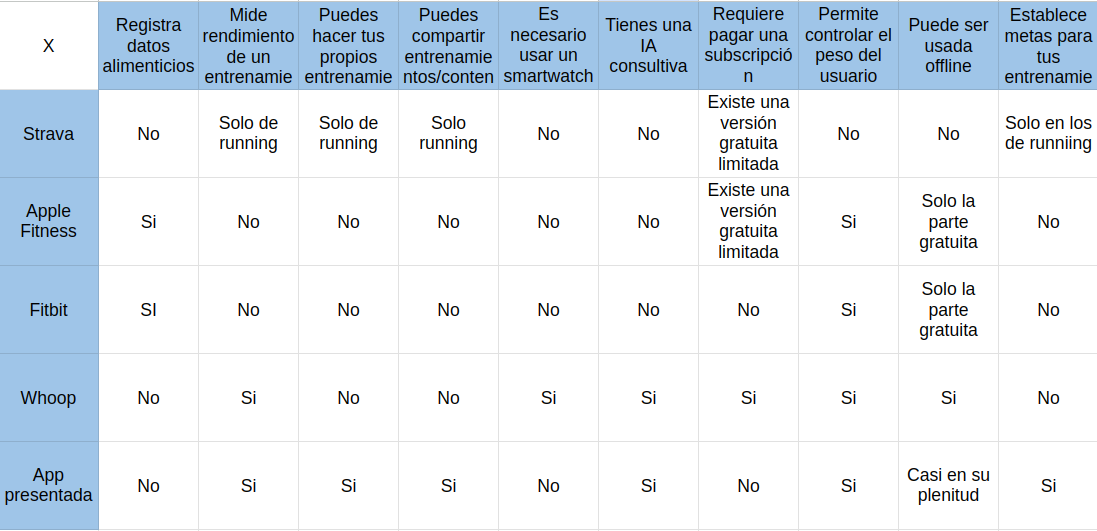
\includegraphics[width=1.65\textwidth]{tablas/tabla.png}
    \caption{Tabla comparativa}
    \label{fig:Tabla comparativa}
\end{figure} 
\end{landscape}

\section{Elección de tecnologías}

\section{Backend}

Se usará Express.js(Node.js), la principal razón que se tiene para optar por esta tecnología, es la gran familiaridad que se tiene con el entorno de JavaScript, se conocen las tecnologías y la forma de implementación, su gran flexibilidad para implementar muchas funcionalidades diversas también fué una buena baza para escoger esta herramienta.
Django fué la primera descartada, porque como bien dice en la tabla de la sección anterior(\cref{fig:Tabla backend}) está más enfocado a proyectos de gran envergadura.
Ruby on Rails fue la que más dudas planteó, como se dijo anteriormente es muy buena opción para las metodologías ágiles y como se dirá más adelante, se optará por una metodología ágil para el desarrollo. Pero al final se descartó por el desconocimiento de la herramienta.

\section{Frontend}

Se ha decidido usar Flutter, dado que Xamarin es buena herramienta, pero está más enfocada a un desarrollo en un ambiente Microsoft.
React Native también es una buena herramienta, fue principalmente la que más dudas sembró, ya que como se dijo previamente se usará un backend basado en Express.js, esto entonces permitiría unificar entornos lo cual favorecería al desarrollo. pero se descartó por lo personalizable que son las IUs desarrolladas en Flutter respecto a esta tecnología.

\section{Base de datos}

Para las bases de datos, tanto para el backend como para la local de la app se usará una SQL, dado a la familiaridad que se dispone con esta tecnología y la necesidad de unificar el tipo de tecnología del servidor y de la app. Esto anterior se debe a que como bien se ha dicho se usará Flutter como entorno frontend y la herramienta que se facilita para el almacenamiento local en este es SQlite, basada en un modelo relacional.

Los modelos NoSQL, se descartaron principalmente porque las relaciones entre elementos suelen ser más complejas y en este proyecto pueden enrevesarse facilmente.

\section{Diagrama de arquitectura}

\begin{figure}[H]
   \centering
    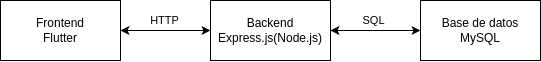
\includegraphics[width=\textwidth]{tablas/Arq.png}
    \caption{Tabla comparativa}
    \label{fig:Tabla comparativa}
\end{figure} 

\section{Metodología utilizada}
Para el desarrollo de esta app, se usará una metodología \textit{ágil} tipo \textbf{SCRUM}. Se decidió usar esta porque permite corregir fallos en la velocidad de diseño y/o planificación de forma eficiente y sin dañar el producto final. Esta metodología permite también entregar desarrollos funcionales a la tutora e ir validando las funcionalidades poco a poco mediante reuniones.

Las reuniones con la tutora serán las \textit{sprint reviews}.

\section{Temporización}
La temporización se realizó el día 25 de marzo de 2025. La entrega del producto (este TFG) está prevista para el 16 de junio de 2025, es decir, 83 días, o lo que es lo mismo, casi 12 semanas. Si un sprint dura 2 semanas, habrá 6 sprints hasta la entrega final.

La iteración 0 se dedicará al diseño de pantallas y al repaso de las funcionalidades de la app, para concretar las historias de usuario y sus prioridades. La idea inicial es dividir la app en varios módulos y centrar cada sprint en cada uno de ellos:

\begin{enumerate}
  \item Ejercicios
  \item Rutinas, usuarios y sesión
  \item Descargar y compartir rutinas
  \item Flujo de entrenamiento
  \item Inteligencia Artificial (IA)
  \item Smartwatch y tratamiento de datos
\end{enumerate}

\section{Seguimiento del desarrollo}

\subsection{Iteración 0}
En esta primera iteración me centré en realizar los diseños de la app, considerando su accesibilidad. También concreté el \textit{product backlog}, compuesto por 41 historias de usuario. En las historias no menciono ningún actor puesto que solo existe el usuario que realiza los ejercicios y el es protagonista en todas ellas, no hay ningún moderador.

A pesar de trabajar con SCRUM se realizarán todos los diseños de interfaces de usuario en este primer sprint para concretar con la tutora los requisitos principales de la aplicación a desarrollar en este TFG. En nuestro caso los diseños de las interfaces se usarán como herramientas de captura y especificación de requisitos. En cada iteración se podrán revisar si hay cambios. 

La lista inicial de historias de usuario es la siguiente, y algunas incluyen tareas secundarias:

\begin{description}
  \item[\textbf{SCRUM-1}] Registrar peso por día
  \item[\textbf{SCRUM-2}] Establecer peso objetivo
  \item[\textbf{SCRUM-3}] Insertar/Borrar/Modificar ejercicio de la lista de ejercicios
  \item[\textbf{SCRUM-4}] Buscar rutina en la lista del usuario
  \item[\textbf{SCRUM-5}] Insertar/Borrar/Modificar rutina
  \item[\textbf{SCRUM-6}] Hacer gráfica en base a las marcas obtenidas
  \item[\textbf{SCRUM-7}] Revisar datos para ver si el descanso es necesario
  \item[\textbf{SCRUM-8}] Enseñar datos de una rutina a descargar
  \item[\textbf{SCRUM-9}] Compartir mi rutina
  \item[\textbf{SCRUM-10}] Valorar el entrenamiento en base a la marca actual y la meta del usuario
  \item[\textbf{SCRUM-11}] Monitorizar pulso en tiempo real
  \item[\textbf{SCRUM-12}] Medir pulso en reposo y compararlo con datos de ejercicios
  \item[\textbf{SCRUM-13}] Avisar de anomalías en el pulso de forma suave
  \item[\textbf{SCRUM-14}] Obtener calorías quemadas
  \item[\textbf{SCRUM-15}] Comprobar el equilibrio nervioso del usuario
  \item[\textbf{SCRUM-16}] Realizar el flujo del entrenamiento
  \item[\textbf{SCRUM-17}] Conectar con la IA para iniciar diálogo
  \item[\textbf{SCRUM-18}] Crear/Borrar usuario
  \item[\textbf{SCRUM-19}] Resumir datos
  \item[\textbf{SCRUM-20}] Iniciar/Cerrar sesión
  \item[\textbf{SCRUM-21}] Medir SpO2
  \item[\textbf{SCRUM-22}] Interpretar constantes
  \item[\textbf{SCRUM-23}] Buscar ejercicios en la lista de ejercicios
  \item[\textbf{SCRUM-24}] Pop up de confirmación
  \item[\textbf{SCRUM-25}] Implementar menú principal
  \item[\textbf{SCRUM-26}] Detectar metas cumplidas en los ejercicios después del entrenamiento
  \item[\textbf{SCRUM-27}] Buscar rutinas para descargar
  \item[\textbf{SCRUM-28}] Implementar calendario
\end{description}


A continuación se muestran los diseños creados en esta iteración:

\textbf{Inicio de sesion y crear usuario}

\begin{figure}[H]
   \centering
    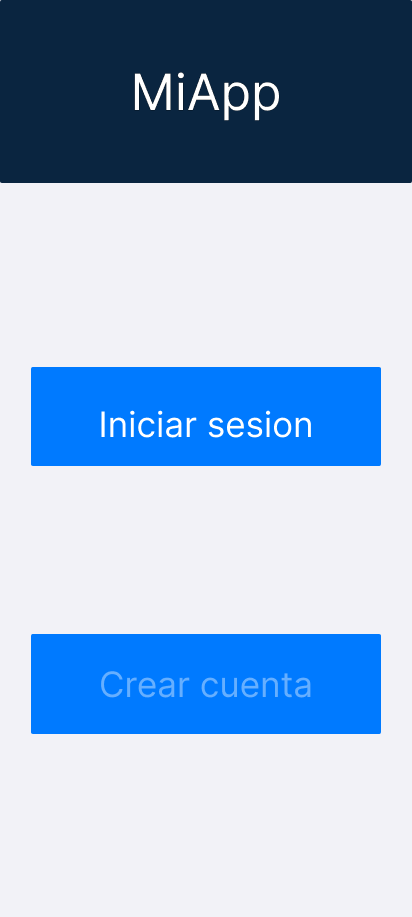
\includegraphics[width=0.6\textwidth]{fotos/Frame 22.png}
    \caption{Pagina inicial}
    \label{fig:Pagina inicial}
\end{figure}
\begin{figure}[H]
   \centering
    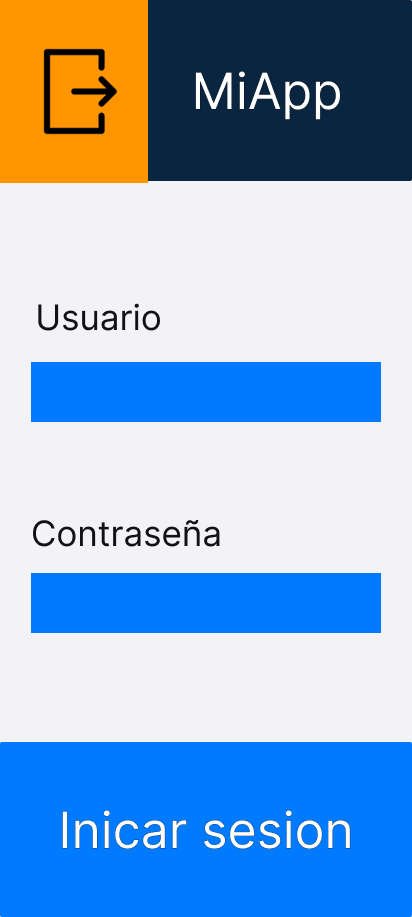
\includegraphics[width=0.6\textwidth]{fotos/Frame 22-1.png}
    \caption{Inicio de sesion}
    \label{fig:Inicio de sesion}
\end{figure}
\begin{figure}[H]
   \centering
    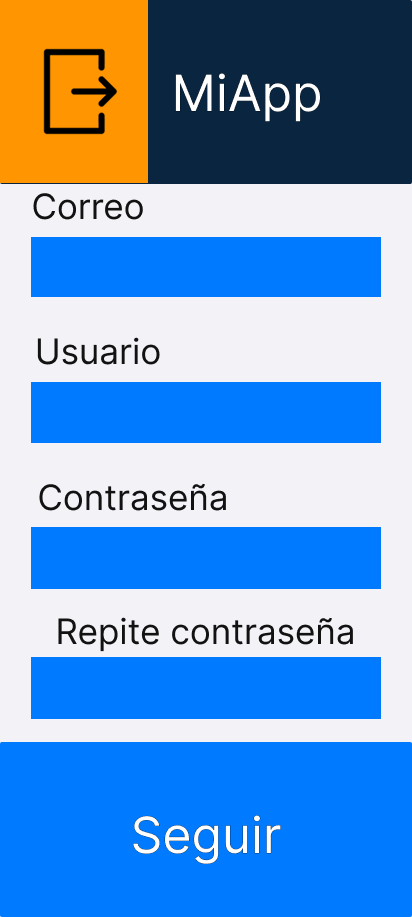
\includegraphics[width=0.6\textwidth]{fotos/Frame 24.png}
    \caption{Crear cuenta 1}
    \label{fig:Crear cuenta 1}
\end{figure}
\begin{figure}[H]
   \centering
    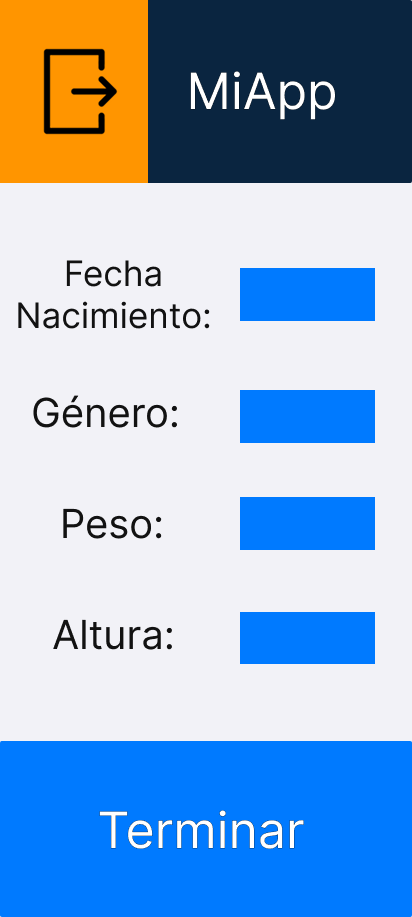
\includegraphics[width=0.6\textwidth]{fotos/Frame 25.png}
    \caption{Crear cuenta 2}
    \label{fig:Crear cuenta 2}
\end{figure}

\textbf{Menu principal}

\begin{figure}[H]
   \centering
    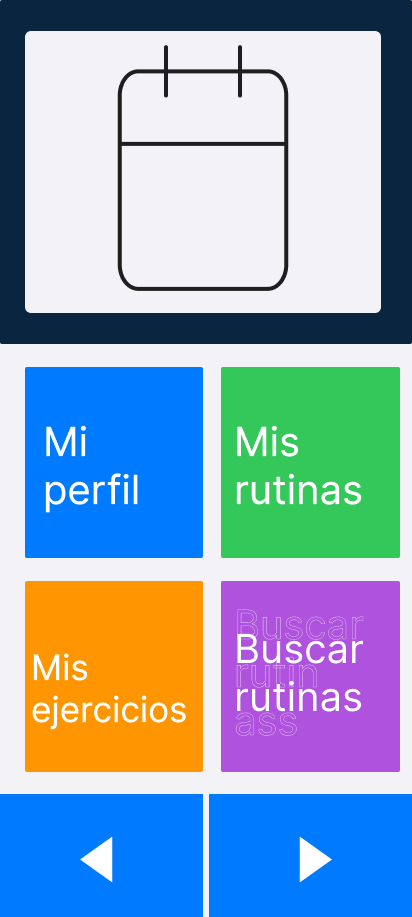
\includegraphics[width=0.6\textwidth]{fotos/Frame 30.png}
    \caption{Menu principal}
    \label{fig:Menu principal}
\end{figure}

\textbf{Lista ejercicios del usuario}

\begin{figure}[H]
   \centering
    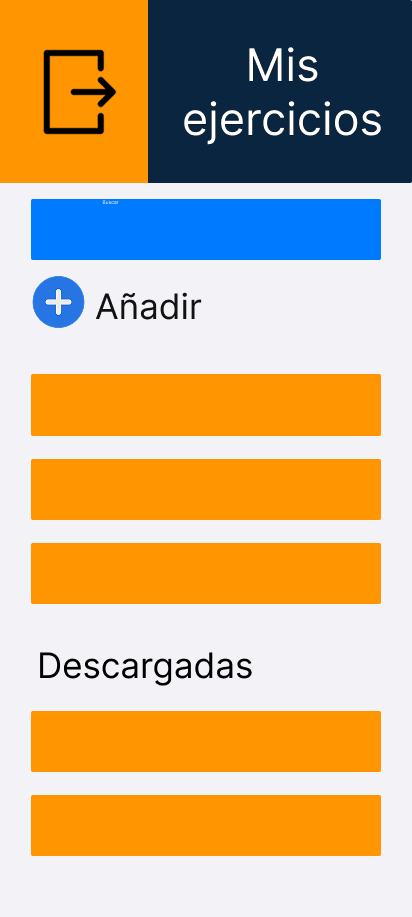
\includegraphics[width=0.6\textwidth]{fotos/Frame 40.png}
    \caption{Lista ejercicios}
    \label{fig:Lista ejercicios}
\end{figure}
\begin{figure}[H]
   \centering
    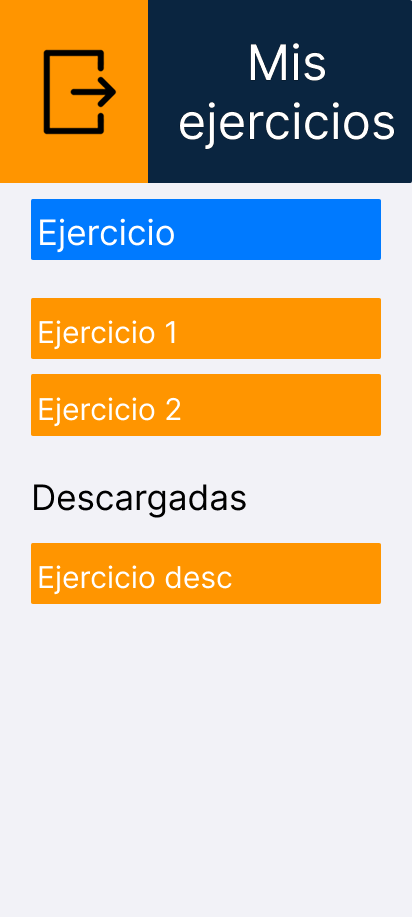
\includegraphics[width=0.6\textwidth]{fotos/Frame 41.png}
    \caption{Lista ejercicios filtrada}
    \label{fig:Lista ejercicios filtrada}
\end{figure}
\begin{figure}[H]
   \centering
    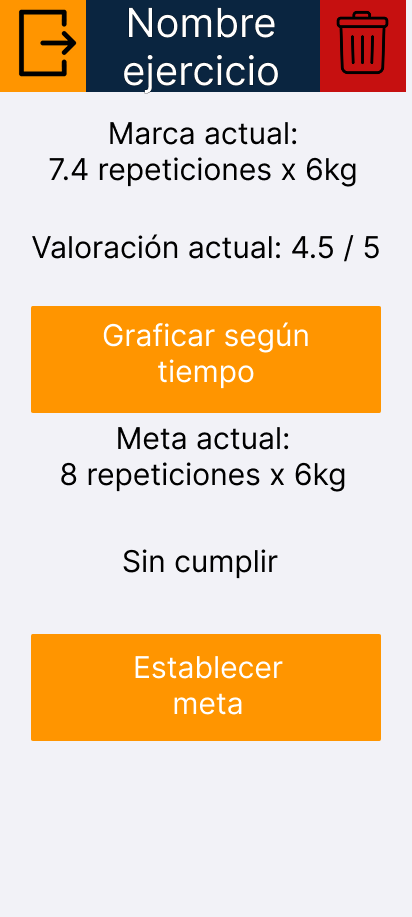
\includegraphics[width=0.6\textwidth]{fotos/Frame 42.png}
    \caption{Datos ejercicio}
    \label{fig:Datos ejercicio}
\end{figure}
\begin{figure}[H]
   \centering
    
\includegraphics[width=0.6\textwidth]{fotos/Frame 43.png}
    \caption{Pop up graficar segun tiempo}
    \label{fig:Pop up graficar segun tiempo}
\end{figure}
\begin{figure}[H]
   \centering
    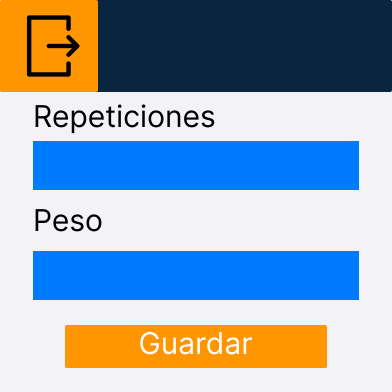
\includegraphics[width=0.6\textwidth]{fotos/Frame 45.png}
    \caption{Pop up establecer meta}
    \label{fig:Pop up establecer meta}
\end{figure}
\begin{figure}[H]
   \centering
    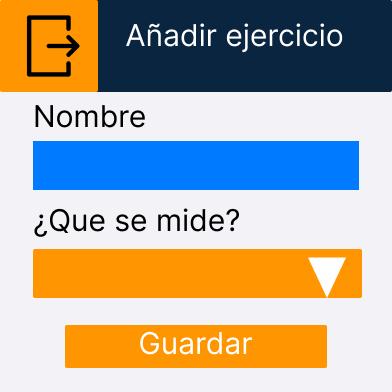
\includegraphics[width=0.6\textwidth]{fotos/Frame 64.png}
    \caption{Pop up crear ejercicio}
    \label{fig:Pop up crear ejercicio}
\end{figure}

\textbf{Lista rutinas}

\begin{figure}[H]
   \centering
    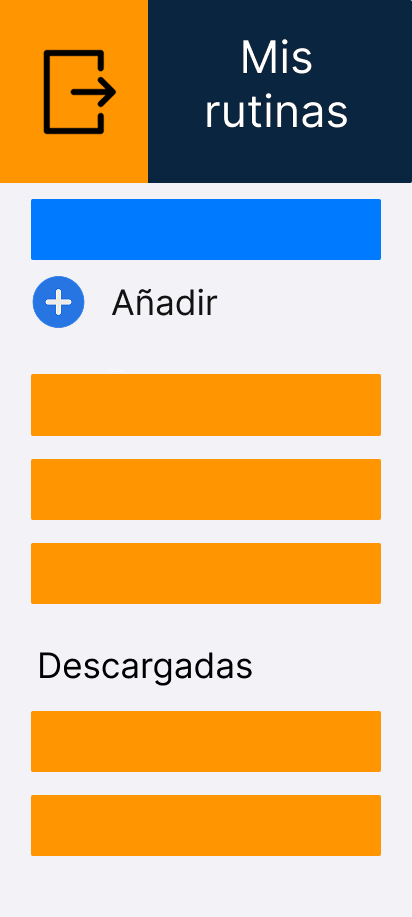
\includegraphics[width=0.6\textwidth]{fotos/Frame 46.png}
    \caption{Lista rutinas}
    \label{fig:Lista rutinas}
\end{figure}
\begin{figure}[H]
   \centering Pop up datos de un ejercicio en entrenamiento
    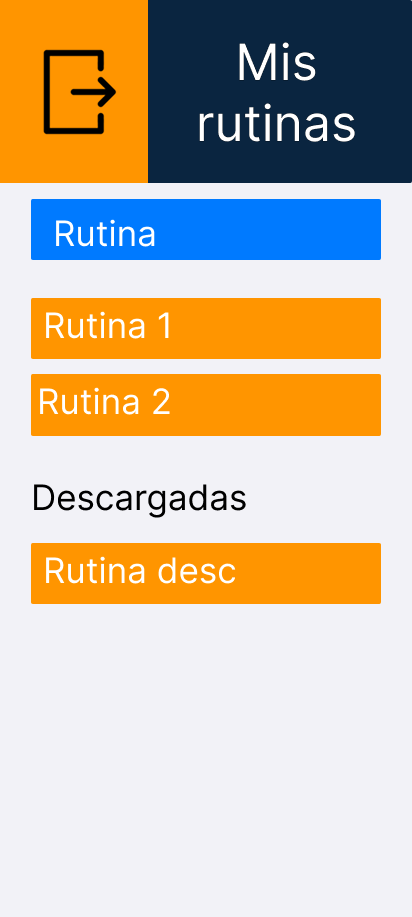
\includegraphics[width=0.6\textwidth]{fotos/Frame 47.png}
    \caption{Lista rutinas filtradas}
    \label{fig:Lista rutinas filtradas}
\end{figure}
\begin{figure}[H]
   \centering
    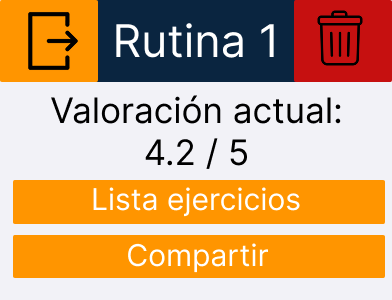
\includegraphics[width=0.6\textwidth]{fotos/Frame 48.png}
    \caption{Datos rutina modificable}
    \label{fig:Datos rutina modificable}
\end{figure}
\begin{figure}[H]
   \centering
    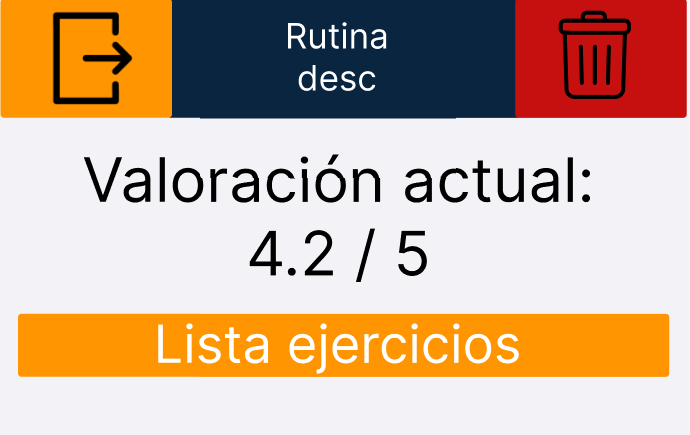
\includegraphics[width=0.6\textwidth]{fotos/Frame 49.png}
    \caption{Datos rutina no modificable}
    \label{fig:Datos rutina no modificable}
\end{figure}
\begin{figure}[H]
   \centering
    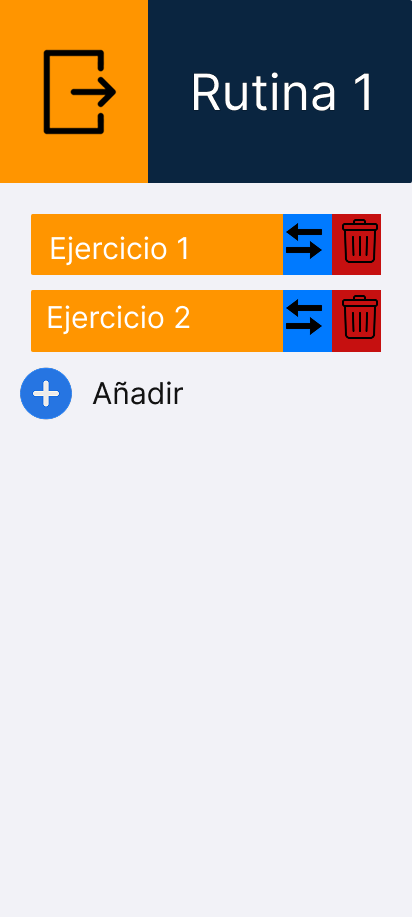
\includegraphics[width=0.6\textwidth]{fotos/Frame 50.png}
    \caption{Modificar ejericios rutina}
    \label{fig:Modificar ejericios rutina}
\end{figure}
\begin{figure}[H]
   \centering
    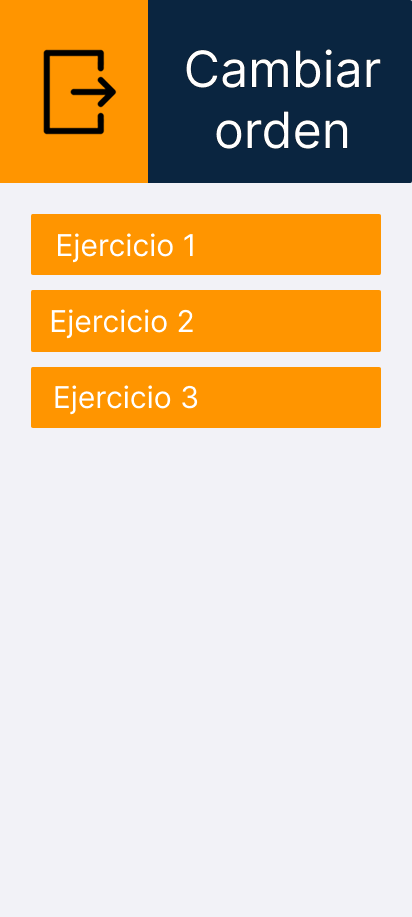
\includegraphics[width=0.6\textwidth]{fotos/Frame 51.png}
    \caption{Cambiar orden ejercicios rutina}
    \label{fig:Cambiar orden ejercicios rutina}
\end{figure}
\begin{figure}[H]
   \centering
    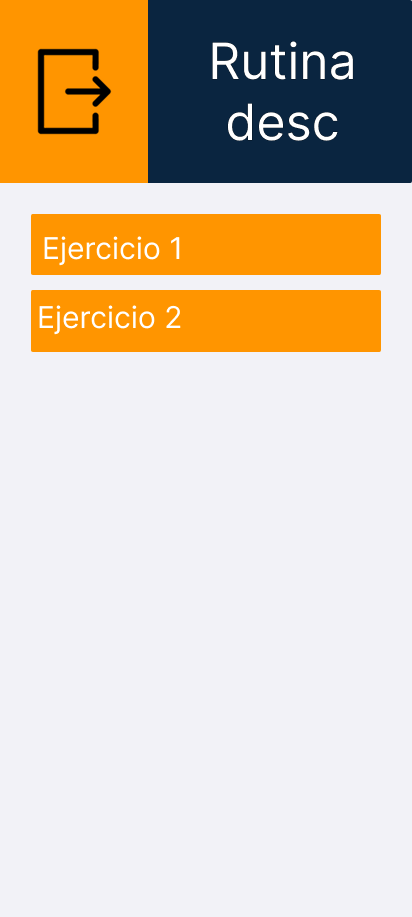
\includegraphics[width=0.6\textwidth]{fotos/Frame 52.png}
    \caption{Ejercicios rutina descargada}
    \label{fig:Ejercicios rutina descargada}
\end{figure}
\begin{figure}[H]
   \centering
    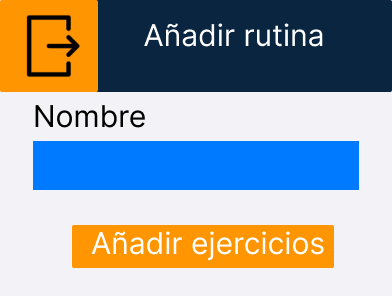
\includegraphics[width=0.6\textwidth]{fotos/Frame 65.png}
    \caption{Pop up crear rutinas}
    \label{fig:Pop up crear rutinas}
\end{figure}

\textbf{Mi perfil}

\begin{figure}[H]
   \centering
    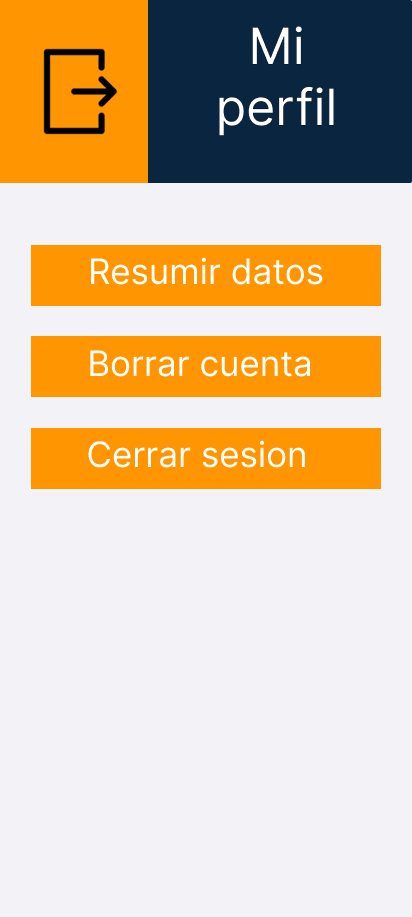
\includegraphics[width=0.6\textwidth]{fotos/Frame 36.png}
    \caption{Opciones de perfil usuario}
    \label{fig:Opciones de perfil usuario}
\end{figure}
\begin{figure}[H]
   \centering
    
\includegraphics[width=0.75\textwidth]{fotos/Frame 38.png}
    \caption{Pop up de confirmacion}
    \label{fig:Pop up de confirmacion}
\end{figure}
\begin{figure}[H]
   \centering
    
\includegraphics[width=0.75\textwidth]{fotos/Frame 39.png}
    \caption{Pop up de confirmacion resumir datos}
    \label{fig:Pop up de confirmacion resumir datos}
\end{figure}

\textbf{Buscar rutina para descargar}

\begin{figure}[H]
   \centering
    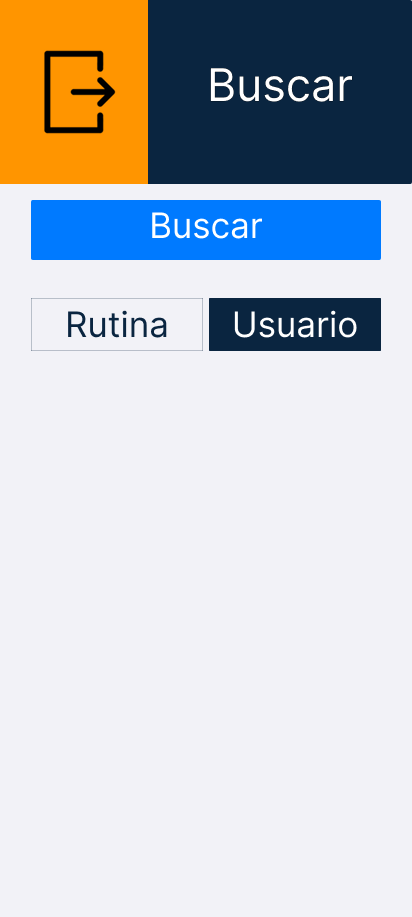
\includegraphics[width=0.6\textwidth]{fotos/Frame 53.png}
    \caption{Buscar usuario}
    \label{fig:Buscar usuario}
\end{figure}
\begin{figure}[H]
   \centering
    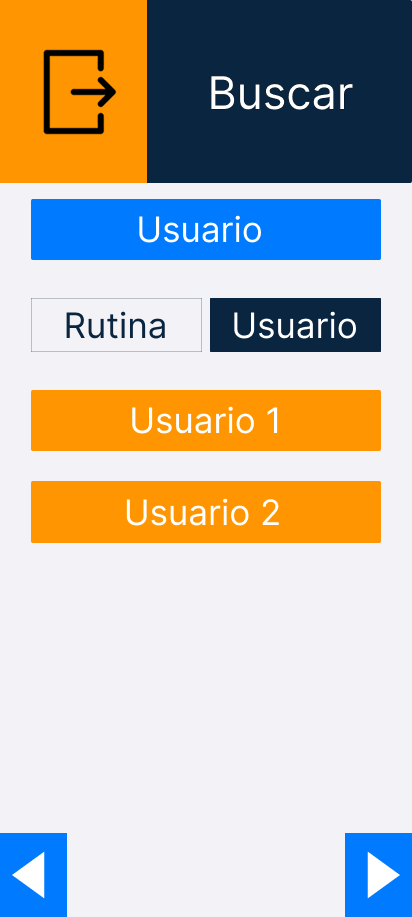
\includegraphics[width=0.6\textwidth]{fotos/Frame 54.png}
    \caption{Buscar usuario filtrado}
    \label{fig:Buscar usuario filtrado}
\end{figure}
\begin{figure}[H]
   \centering
    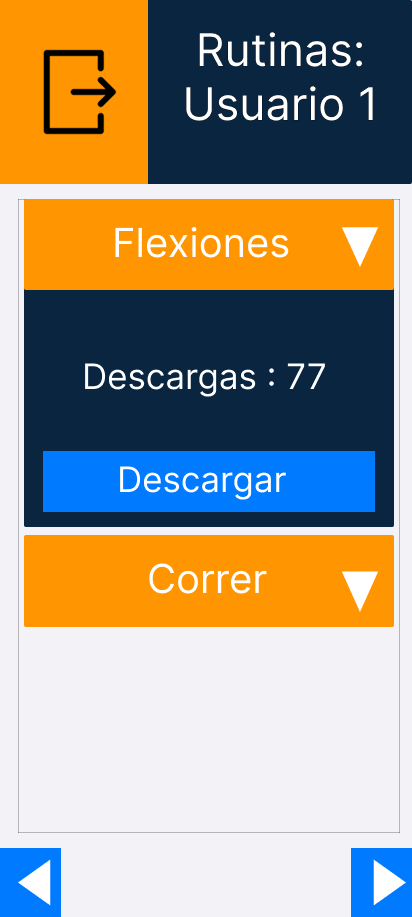
\includegraphics[width=0.6\textwidth]{fotos/Frame 56.png}
    \caption{Rutinas de un usuario}
    \label{fig:Rutinas de un usuario}
\end{figure}
\begin{figure}[H]
   \centering
    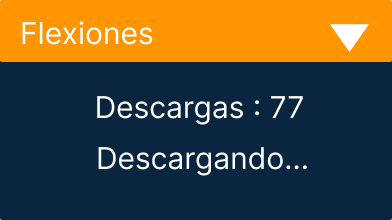
\includegraphics[width=0.6\textwidth]{fotos/Frame 57.png}
    \caption{Widget descargar rutina}
    \label{fig:Widget descargar rutina}
\end{figure}
\begin{figure}[H]
   \centering
    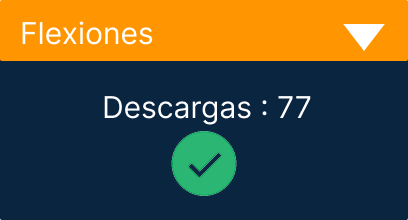
\includegraphics[width=0.6\textwidth]{fotos/Frame 58.png}
    \caption{Widget rutina descargada}
    \label{fig:Widget rutina descargada}
\end{figure}
\begin{figure}[H]
   \centering
    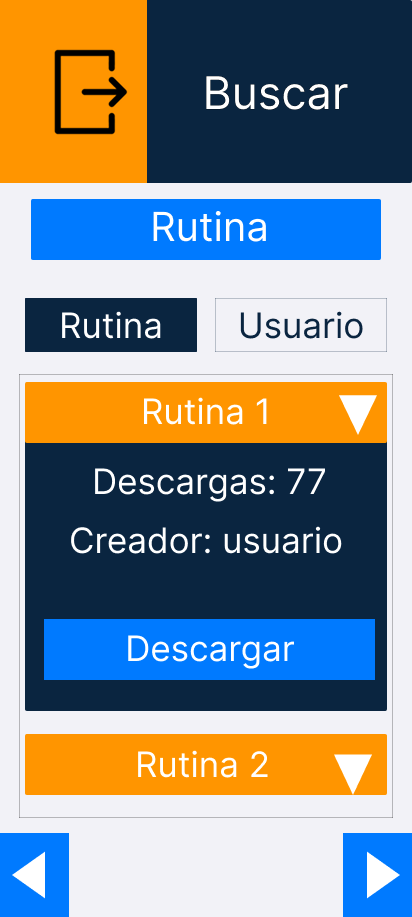
\includegraphics[width=0.6\textwidth]{fotos/Frame 59.png}
    \caption{Buscar rutinas por su nombre filtrada}
    \label{fig:Buscar rutinas por su nombre filtrada}
\end{figure}

\textbf{Entrenamiento (Una vez seleccionada una fecha en el calendario del menu principal saldría la siguiente ventana)}

\begin{figure}[H]
   \centering
    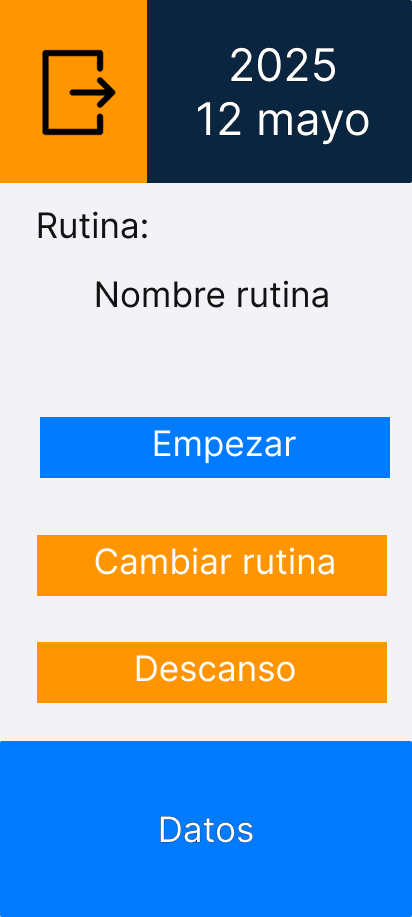
\includegraphics[width=0.6\textwidth]{fotos/Frame 26.png}
    \caption{Entrenamiento de un día determinado}
    \label{fig:Entrenamiento de un día determinado}
\end{figure}
\begin{figure}[H]
   \centering
    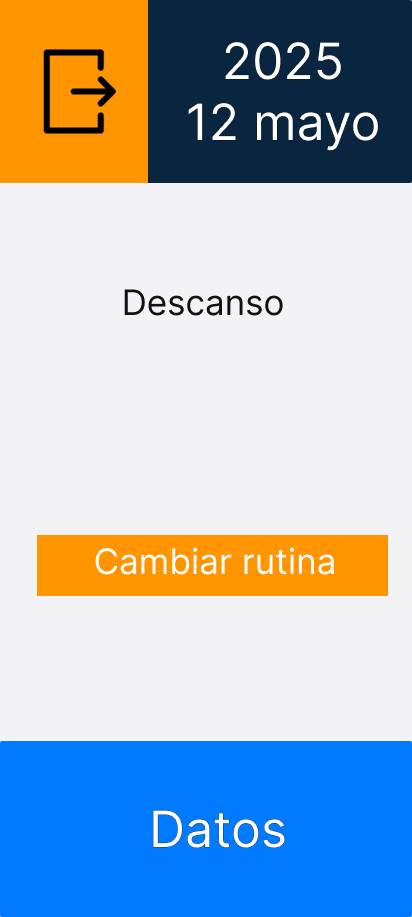
\includegraphics[width=0.6\textwidth]{fotos/Frame 27.png}
    \caption{Descanso en un día determinado}
    \label{fig:Descanso en un día determinado}
\end{figure}

Si seleccionamos datos de una fecha saldría esto
\begin{figure}[H]
   \centering
    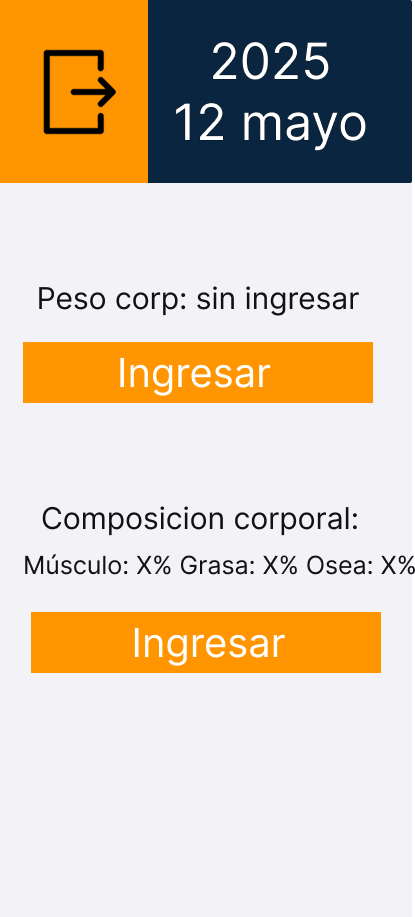
\includegraphics[width=0.6\textwidth]{fotos/Frame 29.png}
    \caption{Frame 29.png}
    \label{fig:Frame_29}
\end{figure}

La siguiente pantalla sale al comenzar el entrenamiento
\begin{figure}[H]
   \centering
    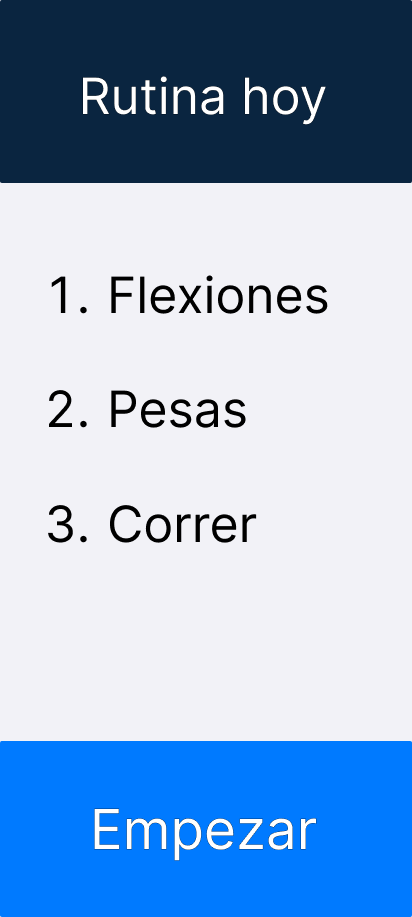
\includegraphics[width=0.6\textwidth]{fotos/Frame 1.png}
    \caption{Lista ejercicios del entrenamiento actual}
    \label{fig:Lista ejercicios del entrenamiento actual}
\end{figure}
\begin{figure}[H]
   \centering
    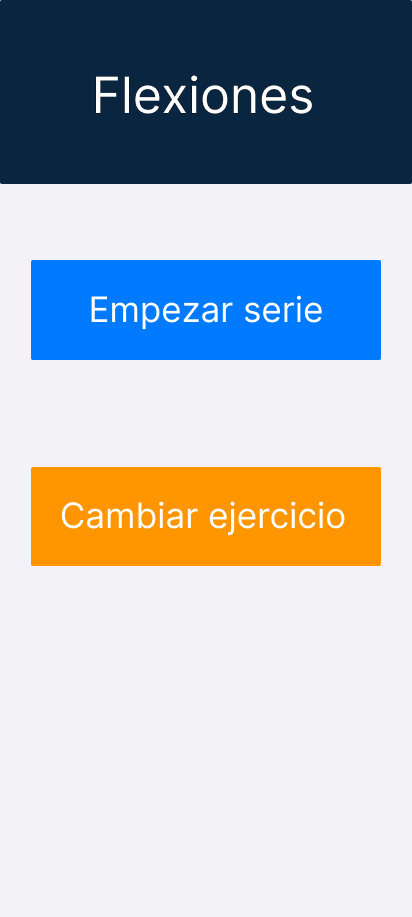
\includegraphics[width=0.6\textwidth]{fotos/Frame 2.png}
    \caption{Primera serie flexiones}
    \label{fig:Primera serie flexiones}
\end{figure}
\begin{figure}[H]
   \centering
    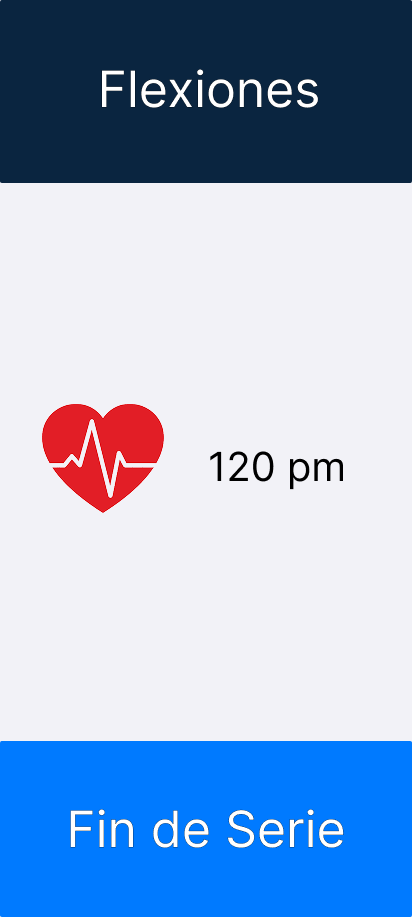
\includegraphics[width=0.6\textwidth]{fotos/Frame 3.png}
    \caption{Realizando flexiones}
    \label{fig:Realizando flexiones}
\end{figure}
\begin{figure}[H]
   \centering
    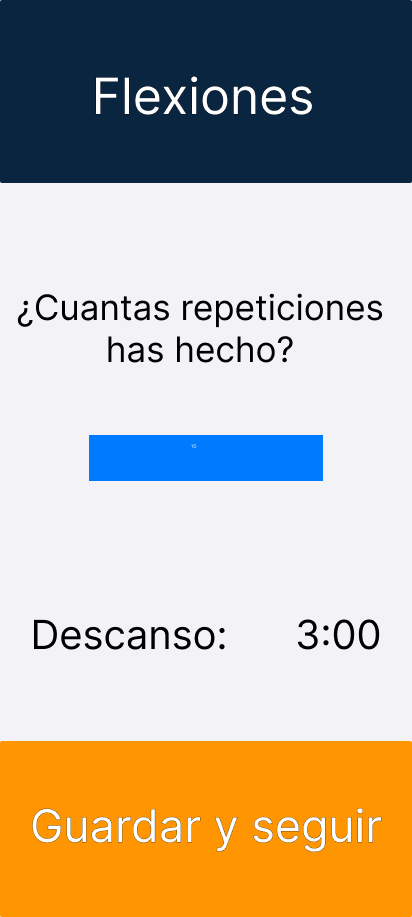
\includegraphics[width=0.6\textwidth]{fotos/Frame 4.png}
    \caption{Fin de la serie(Descanso no completado)}
    \label{fig:Fin de la serie(Descanso no completado)}
\end{figure}
\begin{figure}[H]
   \centering
    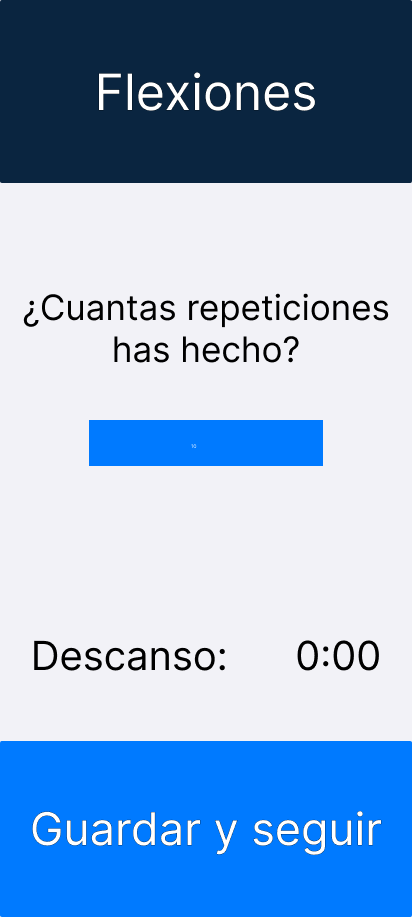
\includegraphics[width=0.6\textwidth]{fotos/Frame 5.png}
    \caption{Fin de la serie(Descanso completado)}
    \label{fig:Fin de la serie(Descanso completado)}
\end{figure}
\begin{figure}[H]
   \centering
    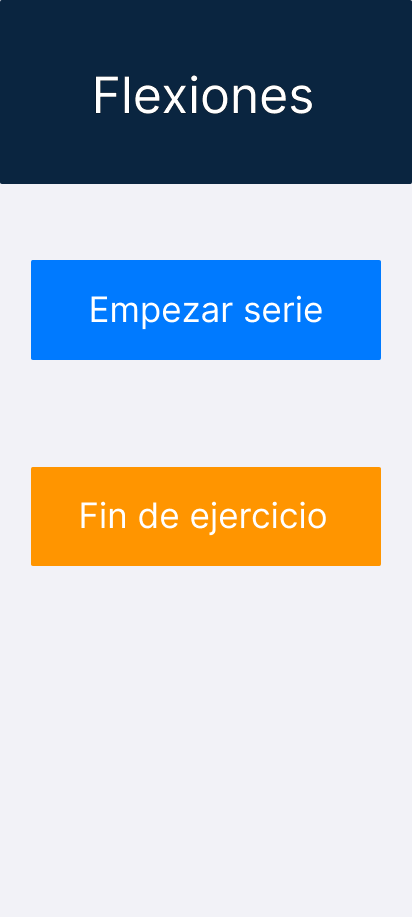
\includegraphics[width=0.6\textwidth]{fotos/Frame 62.png}
    \caption{Acabar ejercicio o añadir serie}
    \label{fig:Acabar ejercicio o añadir serie}
\end{figure}
\begin{figure}[H]
   \centering
    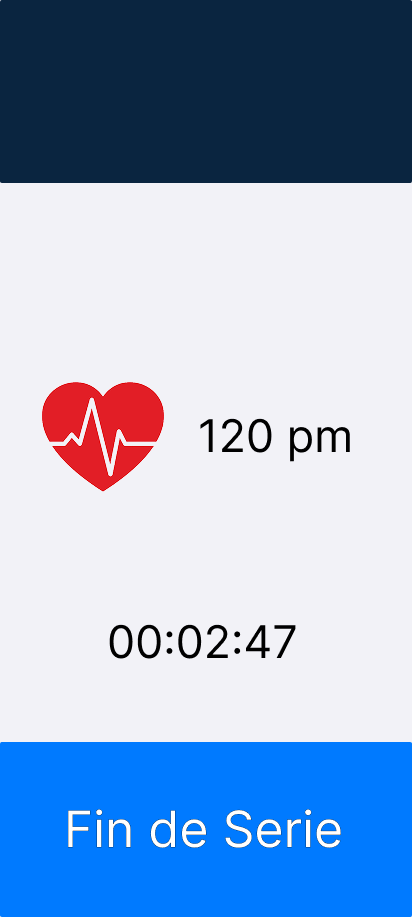
\includegraphics[width=0.6\textwidth]{fotos/Frame 60.png}
    \caption{Realizando ejercicio midiendo tiempo}
    \label{fig:Realizando ejercicio midiendo tiempo}
\end{figure}
\begin{figure}[H]
   \centering
    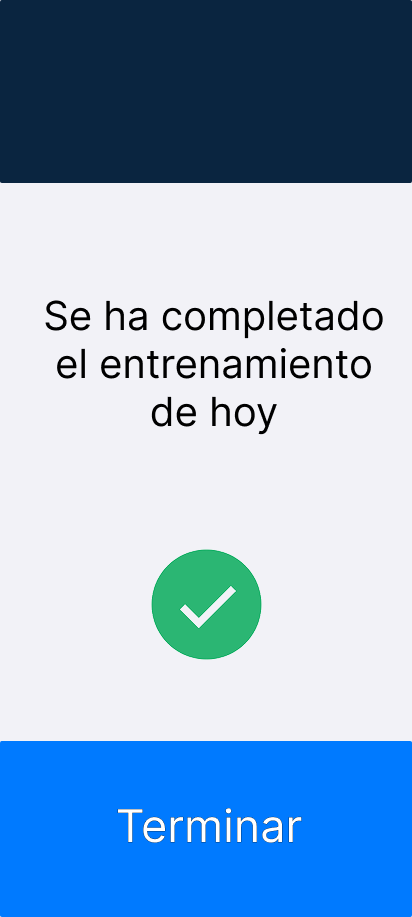
\includegraphics[width=0.6\textwidth]{fotos/Frame 20.png}
    \caption{Fin entrenamiento}
    \label{fig:Fin entrenamiento}
\end{figure}
\begin{figure}[H]
   \centering
    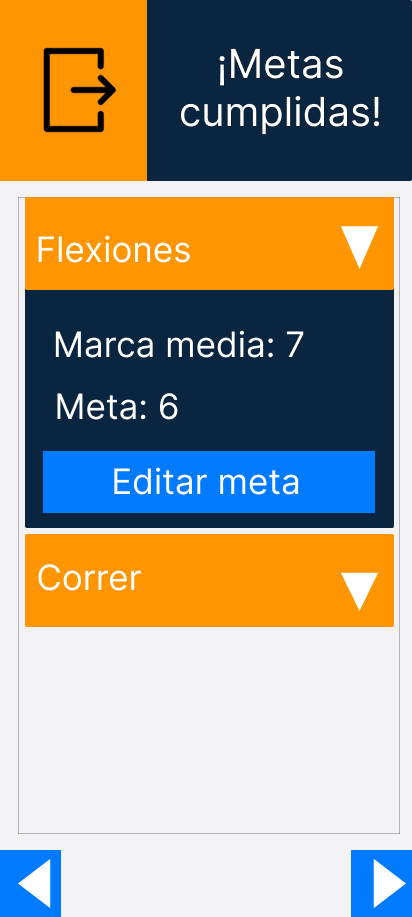
\includegraphics[width=0.6\textwidth]{fotos/Frame 37.png}
    \caption{Metas cumplidas}
    \label{fig:Metas cumplidas}
\end{figure}
\begin{figure}[H]
   \centering
    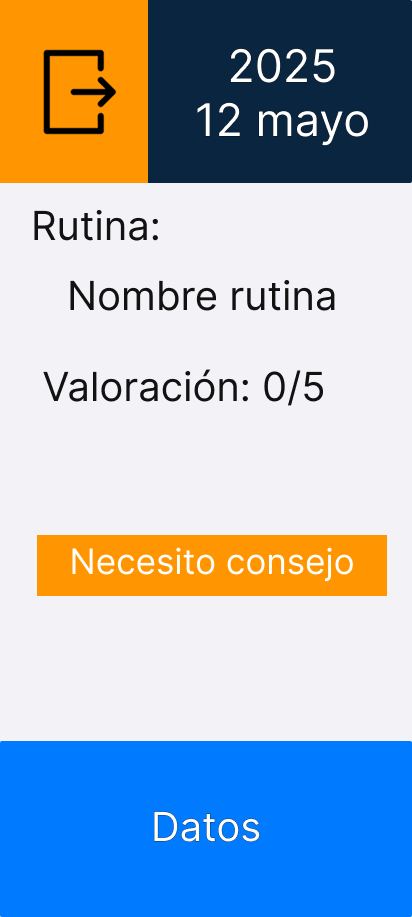
\includegraphics[width=0.6\textwidth]{fotos/Frame 31.png}
    \caption{Datos entrenamiento terminado}
    \label{fig:Datos entrenamiento terminado}
\end{figure}

El chat de la IA se abre cuando se le da a la opcion necesito consejo de un entrenamiento realizado
\begin{figure}[H]
   \centering
    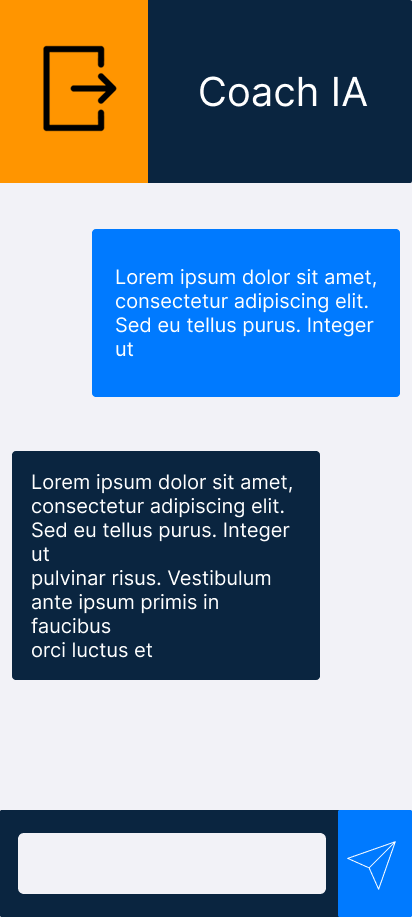
\includegraphics[width=0.6\textwidth]{fotos/Frame 32.png}
    \caption{Chat con IA}
    \label{fig:Chat con IA}
\end{figure}

Si le das a datos de un entrenamiento terminado
\begin{figure}[H]
   \centering
    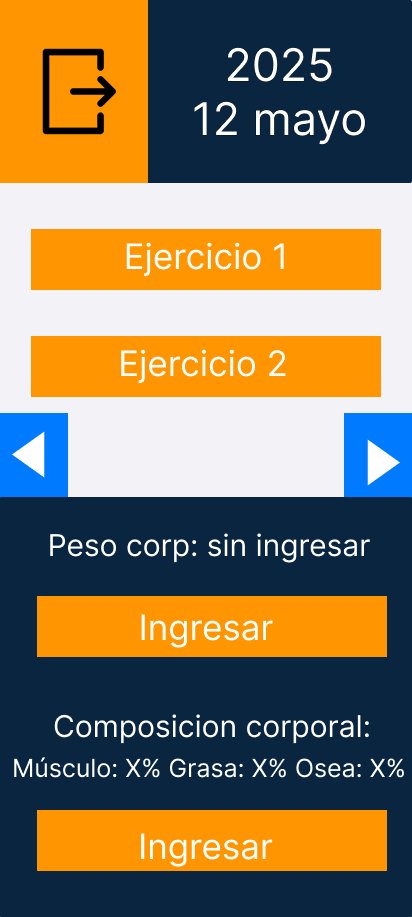
\includegraphics[width=0.6\textwidth]{fotos/Frame 33.png}
    \caption{Datos detallados entrenamiento terminado}
    \label{fig:Datos detallados entrenamiento terminado}
\end{figure}
\begin{figure}[H]
   \centering
    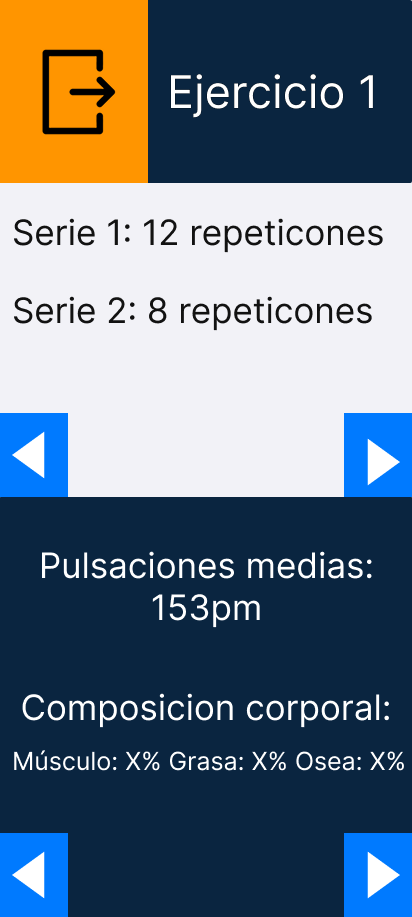
\includegraphics[width=0.6\textwidth]{fotos/Frame 35.png}
    \caption{Pop up datos de un ejercicio en entrenamiento}
    \label{fig:Pop up datos de un ejercicio en entrenamiento}
\end{figure}


Estos diseños pueden cambiar y sufrir alteraciones debido a los sprints reviews y correcciones de accesibilidad. De todas formas, cada cambio será informado con su motivo.

\subsubsection{Sprint Review 0}
Durante esta revisión de sprint se realizaron mejoras de diseño, como la incorporación de iconos en todos los botones para mejorar la accesibilidad. Se revisaron también los títulos de las ventanas, cambiando aquellos que no eran lo suficientemente claros.

Además, se añadieron nuevas historias al \textit{product backlog}, incorporando o desglosando funcionalidades:

\begin{itemize}
  \item SCRUM-29: Copiar rutina
  \item SCRUM-30: Añadir meta por parámetro
  \item SCRUM-31: Solicitar permiso al usuario antes de enviar datos a la IA
  \item SCRUM-32: Enviar datos del entrenamiento actual y anteriores a la IA
  \item SCRUM-33: Conectar/Desconectar con la IA
\end{itemize}

El backlog quedaría de la siguiente manera:

\begin{landscape}
\begin{figure}[H]
   \centering
    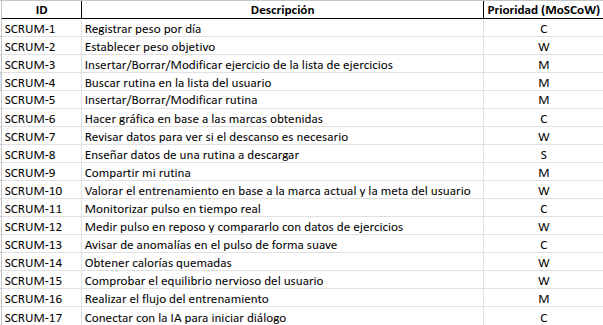
\includegraphics[width=1.5\textwidth]{tablas/backlog1.png}
    \caption{Backlog prioridades MoSCoW}
    \label{fig:backlog1}
\end{figure}
\end{landscape}

\begin{landscape}
\begin{figure}[H]
   \centering
    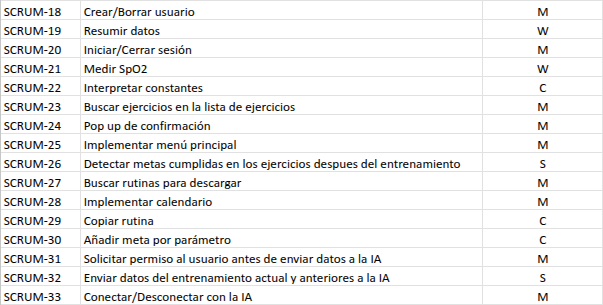
\includegraphics[width=1.5\textwidth]{tablas/backlog2.png}
    \caption{Backlog prioridades MoSCoW}
    \label{fig:backlog2}
\end{figure}
\end{landscape}

\begin{figure}[H]
   \centering
    \includegraphics[width=1.2\textwidth]{tablas/iter1.png}
    \caption{Iteracion 1}
    \label{fig:iter1}
\end{figure}

\begin{figure}[H]
   \centering
    \includegraphics[width=1.1\textwidth]{tablas/iter2.png}
    \caption{Iteracion 2}
    \label{fig:iter2}
\end{figure}

\begin{figure}[H]
   \centering
    \includegraphics[width=1.2\textwidth]{tablas/iter3.png}
    \caption{Iteracion 3}
    \label{fig:iter3}
\end{figure}

\begin{figure}[H]
   \centering
    \includegraphics[width=1.25\textwidth]{tablas/iter4.png}
    \caption{Iteracion 4}
    \label{fig:iter4}
\end{figure}

\begin{figure}[H]
   \centering
    \includegraphics[width=1.25\textwidth]{tablas/iter5.png}
    \caption{Iteracion 5}
    \label{fig:iter5}
\end{figure}

\begin{figure}[H]
   \centering
    \includegraphics[width=1.25\textwidth]{tablas/iter6.png}
    \caption{Iteracion 6}
    \label{fig:iter6}
\end{figure}

\subsection{Iteración 1}
La lista de historias de la primera iteracion queda de la siguiente manera:

\begin{itemize}
    \item SCRUM-23: Buscar ejercicio en lista de ejercicios
    \item SCRUM-3: Insertar/Borrar/Modificar ejercicio de la lista de ejercicios
    \item SCRUM-24: Pop up de confirmación
    \item SCRUM-30: Añadir meta por parámetro
\end{itemize}

A continuación especificaremos las tareas y pruebas de cada historia, y los resultados asociados a cada una. 

\HU{
SCRUM-23: Buscar ejercicio en lista de ejercicios
}{
	\item Implementar la BD local
    \item Implementar algoritmo de búsqueda por nombre
   	\item Implementar boceto de IU \cref{fig:Lista ejercicios}
}{
	\item si no existe ejercicio buscado, no sale nada en pantalla
   	\item si existe ejercicio buscado, sale un acceso en pantalla
}

\begin{figure}[H]
   \centering
    \includegraphics[width=0.8\textwidth]{pantallas/listaEjercicios.png}
    \caption{Lista ejercicios}
    \label{fig:ListaEjer}
\end{figure}

Una de las dificultades de esta funcionalidad fue que esta pantalla debería funcionar como una plantilla, es decir, la lista de elementos como una lista de Strings y las función para el acceso a cada elemento, de esta forma se recilclaría mucho código ahorrando tiempo. Lo que se hizo fue una ingeniería inversa, se desarrollo la pantalla forma específica para los ejericios y cuando funcionaba correctamente, se fue abstrayendo el código hasta obtener la clase ListaBusquedaAniadir, la cual tiene elo comportamiento deseado de una plantilla.

Otro problema encontrado durante las pruebas fue la actualización de la lista, se tuvieron muchos problemas dado que en flutter si se tiene una instancia de un widget llamemoslo A, que forma parte de otro llamado B, si yo llamo a una actualización de la IU desde B porque ha cambiado el contenido se genera una excepción. Como solución, se optó por solo usar la función setState (Usada para actualizar el contenido) dentro del código de la plantilla y cada vez que fuera necesario hacer una actualización desde B recargar otra vez la pantalla entera.

El algorítmo de búsqueda funciona de la siguiente manera, digamos que se busca el ejercicio "flexiones" en la lista, entonces se pasa a minúscula todos los elementos de la lista, se pasa la cadena "flexiones" a minúscula y se obtiene como resultado los elementos de la lista que contengan la cadena "flexiones".

Esta funcionalidad pasó todas las pruebas.

\HU{
SCRUM-3: Insertar/Borrar/Modificar ejercicio de la lista de ejercicios
}{
	\item Implementar la BD local
	\item Implementar las funciones para las consultas
	\item Implementar las funciones para las modificaciones
	\item Implementar las funciones para el borrado
	\item Implementar boceto de la IU \cref{fig:Datos ejercicio}, para borrar/modificar desde ahí
}{
	\item si se borra un ejercicio, no sale en la lista
	\item si se modifica, sale con los datos modificados
	\item si se inserta, sale en la lista el ejercicio
	\item se enseñan los datos del ejercicio de forma correcta
}

\begin{figure}[H]
   \centering
    \includegraphics[width=0.8\textwidth]{pantallas/CrearEjercicio.png}
    \caption{Crear ejercicios}
    \label{fig:CrearEjers}
\end{figure}

\begin{figure}[H]
   \centering
    \includegraphics[width=0.8\textwidth]{pantallas/ModDescpEjer.png}
    \caption{Modificar descripcion ejercicios}
    \label{fig:ModDescpEjer}
\end{figure}

Pasó todas las pruebas.

\HU{
SCRUM-30: Añadir meta por parámetro
}{
	\item Implementar la BD local
	\item Implementar las funciones para modificar metas
}{
	\item si existe una meta determinada para ese ejercicio y se quiere insertar una, sustituir la actual
	\item si se insertan los valores en formato incorrecto, informar de errores
	\item si se insertan los valores en formato correcto, guardar
}

\begin{figure}[H]
   \centering
    \includegraphics[width=0.8\textwidth]{pantallas/NuevaMeta.png}
    \caption{Nueva meta}
    \label{fig:NuevaMeta}
\end{figure}

El problema de esta funcionalidad está en interpretar si un usuario quiere superar su meta u obtener una marca menor. Al final se optó por solo interpretar que se pueda superar la marca.

Cabe aclarar una cosa respeto a los formatos de los datos guardados en las metas y las marcas, se guardan 4 tipos de datos repeticiones (entero), peso (decimal), tiempo (tiempo) y distancia (decimal). Para ahorrar espacio en el almacenamiento local, ya que habra mucho volument ocupado en memoria si el usuario sigue usando la app, los datos en formato decimal se suben como un entero, se hace la conversion numeroEntero=(numeroDecimal*100).toInt() se guarda en ese formato y luego al sacarlo de memoria se le hace la conversión inversa.

Pasó todas las pruebas.

\HU{
	SCRUM-24: Pop up de confirmación  
}{
	\item Implementar la confirmación para que pueda ser usado en pantallas distintas
	\item Implementar boceto de IU \cref{fig:Pop up de confirmacion} 
}{
	\item si se ha seleccionado una opcion, se devuelve la opcion seleccionada
}

\begin{figure}[H]
   \centering
    \includegraphics[width=0.8\textwidth]{pantallas/PopUpConfirmacion.png}
    \caption{PopUp Confirmacion}
    \label{fig:PopUpConfirmacion}
\end{figure}

Es un pop up que se usará siempre que se requiera una confirmación ,se implementó para que pueda ser usado en cualquier contexto de la app, pasó las pruebas.

\subsubsection{Estado de la BD local}

Cabe aclarar que la BD local es la memoria persistente de la app que solo existe en el dispositivo que esta instalada la app, se le llama BD local porque tiene una estrucura tipo SQL.

Al finalizar esta iteración, el estado de la BD queda tal y como se muestra en la figura \cref{fig:BD local iteracion 1}
\begin{figure}[H]
   \centering
    \includegraphics[width=\textwidth]{fotos/BDL iteracion 1.png}
    \caption{BD local iteracion 1}
    \label{fig:BD local iteracion 1}
\end{figure}

\subsubsection{Sprint Review 1}
Las primeras iteraciones tienden a ser más lentas debido a la fase inicial del desarrollo. No se completó la totalidad del sprint; quedó pendiente la subtarea de modificar ejercicio en la base de datos(SCRUM-3: Insertar/Borrar/Modificar ejercicio de la lista de ejercicios). Aun así, las expectativas son positivas, ya que se espera un aumento en la velocidad de desarrollo.

La pantalla en la que se enseñan los datos de un ejercicio se modificó para facilitar su lectura y entendimiento, dado que su anterior diseño era confuso.

Otra parte a modificar es la del pop up de confirmación, ya que debido a la poca accesibilidad de los pop ups se sustituirá por una pantalla independiente.

\begin{figure}[h!]
  \centering
  \begin{minipage}[b]{0.45\textwidth}
    \centering
    \includegraphics[width=\textwidth]{fotos/ejerciciosNueva.png}
    \caption{Pantalla nueva}
    \label{fig:pantalla_nueva}
  \end{minipage}
  \hfill
  \begin{minipage}[b]{0.45\textwidth}
    \centering
    \includegraphics[width=\textwidth]{fotos/ejerciciosVieja.png}
    \caption{Pantalla antigua}
    \label{fig:pantalla_vieja}
  \end{minipage}
  \caption{Comparación entre la pantalla nueva y la anterior}
  \label{fig:comparacion_pantallas}
\end{figure}

También se cambiaron todos los pop ups y se sustituyeron por pantallas completas:

\begin{itemize}
	\item Los pop ups de confirmacion
	\item Crear ejercicios
	\item Modificar ejercicios
	\item Nueva meta en un ejercicio
	\item Crear rutinas
	\item Modificar rutinas
	\item Modificar ejercicios de una rutina
	\item Información de una rutina a descargar
	\item Modificar informacion del perfil del usuario
\end{itemize}

Por consecuencia las futuras funcionalidades en la que se mencionan los pop ups, pasaran a ser pantallas completas.

\subsection{Iteración 2}
Esta iteración se centró en el desarrollo del sistema de sesiones, la API de la aplicación, el backend básico del servidor y la sección de rutinas. Las historias que incluye son las siguientes:

\begin{itemize}
  \item SCRUM-18 Crear/Borrar mi usuario
  \item SCRUM-20 Iniciar/Cerrar sesión
  \item SCRUM-5 Insertar/Borrar/Modificar rutina
  \item SCRUM-4 Buscar rutina en la lista del usuario
  \item SCRUM-25 Implementar menú principal
\end{itemize}

También se terminará la historia no finalizada de la iteración anterior(SCRUM-3: Insertar/Borrar/Modificar ejercicio de la lista de ejercicios).

\HU{
SCRUM-25 Implementar menú principal
}{
	\item Implementar el boceto IU \cref{fig:Menu principal}
	\item Añadir accesos a las funcionalidades actuales
}{
	\item si la funcionalidad seleccionada no está implementada, no hacer nada
	\item si la funcionalidad seleccionada está implementada, desplegar ventana de dicha funcionañidad
}

\begin{figure}[H]
   \centering
    \includegraphics[width=0.8\textwidth]{pantallas/MenuPrincipalSemi.png}
    \caption{Menu Principal semifuncional}
    \label{fig:MenuPrincipalSemi}
\end{figure}

Pasó todas las pruebas.

\HU{
SCRUM-18 Crear/Borrar mi usuario
}{
	\item Implementar bocetos de IU \cref{fig:Crear cuenta 1} ,\cref{fig:Crear cuenta 2}, \cref{fig:Pagina inicial} y la parte necesaria de \cref{fig:Opciones de perfil usuario}
	\item Implementar funciones de inserccion y borrado en el backend
}{
	\item si el usuario que se quiere crear ya existe, informar y pedir que se rellenen los credenciales otra vez
	\item si el usuario que se quiere crear no existe, crear usuario y pasar a la siguiente pantalla
	\item si cualquier dato requerido está en un formato incorrecto ,informar al usuario para que vuelva a rellenar estos
	\item si todos los datos están en el formato correcto ,seguir con la creación del usuario
	\item si se ha creado exitosamente el usuario, volver a la pantalla inicial
	\item si se borra el usuario, borrar el token en el dispositvo y sus credenciales en el backend
}

\begin{figure}[H]
   \centering
    \includegraphics[width=0.8\textwidth]{pantallas/LogSingIn.png}
    \caption{Log In / Sing In}
    \label{fig:LogSingIn}
\end{figure}

\begin{figure}[H]
   \centering
    \includegraphics[width=0.8\textwidth]{pantallas/SingIn1.png}
    \caption{Sing In pantalla 1}
    \label{fig:SingIn1}
\end{figure}

\begin{figure}[H]
   \centering
    \includegraphics[width=0.8\textwidth]{pantallas/SingIn2.png}
    \caption{Sing In pantalla 2}
    \label{fig:SingIn2}
\end{figure}

Cabe decir que siempre que se crea un usuario se crea un archivo para almacenar su BD con el nombre del propio usuario. De esta forma separamos el almacenamiento local de los usuarios.

Pasó todas las pruebas.

\HU{
SCRUM-20 Iniciar/Cerrar sesión
}{
	\item Implementar el boceto IU \cref{fig:Inicio de sesion} y parte necesaria de \cref{fig:Opciones de perfil usuario}
	\item Implementar función de consulta en el backend
}{
	\item si el usuario con esa contraseña no existe, informar al usuario
	\item si el usuario con esa contraseña existe, devolver un token para su guardado y guardar usuario 
	\item si el usuario quiere cerrar sesión, borrar token y nombre del usuario del dispositivo y volver a la pantalla inicial \cref{fig:Pagina inicial}
}

\begin{figure}[H]
   \centering
    \includegraphics[width=0.8\textwidth]{pantallas/LogIn.png}
    \caption{Log In}
    \label{fig:LogIn}
\end{figure}

\begin{figure}[H]
   \centering
    \includegraphics[width=0.8\textwidth]{pantallas/OpcUser.png}
    \caption{Opciones Usuario}
    \label{fig:Opciones Usuario}
\end{figure}

Al hacer el login correctamente se otorga un token que no hay que renovar hasta el día siguiente, al cerrar sesión se borra automaticamente. Las pruebas realizadas se basaron en comprobar el correcto alamacenaje y borrado del token, usando la librería de secure storage de flutter, que nos permite guardar variables de forma permanente y encriptada con un facil acceso, como si fuera un map.

Para comprobar la veracidad de los credenciales se implementó la parte básica del backend, un server con una BD(mySQL) que guardará los usuarios con sus contraseñas y la parte implementada usando Express.js(Node.js) para escuchar peticiones, el server también será el encargado de proporcionar y verificar los tokens. La comunicación entre servidor y cliente (el dispositivo en el que esta instalada la app) se usan peticiones HTTP, en futuro se puede migrar a HTTPS si es necesaria mas seguridad.

Se hicieron pruebas abriendo y cerrando sesión comprando si exsitía el token en memoria e intentando acceder a la app usando un token caducado. Siempre se añadía/borraba el token cuando se iniciaba/cerraba sesión y no dejaba entrar usando tokens caducados. Pasó todas las pruebas.

\HU{
SCRUM-4 Buscar rutina en la lista del usuario
}{
	\item Implementar IU del boceto \cref{fig:Lista rutinas}
	\item Implementar lo necesario en la BD local
	\item Implementar algorítmo de búsqueda
	\item Implementar acceso a la rutina seleccionada
}{
	\item si no existe la rutina buscada, no enseñar acceso en pantalla
	\item si existe la rutina buscada, enseñar acceso en pantalla
}

\begin{figure}[H]
   \centering
    \includegraphics[width=0.8\textwidth]{pantallas/listaRutinas.png}
    \caption{Lista Rutinas}
    \label{fig:listaRutinas}
\end{figure}

Esta funcionalidad se abarcó aprovechando lo implementado en la iteración anterior del SCRUM-23. Se realizaron las mismas pruebas pero relacionadas con las rutinas. Como la funcionalidad previamente mencionada se diseñó para poder usar código a modo de plantilla y pasó todas las pruebas, esta como era de esperar las pasó también.

\HU{
SCRUM-5 Insertar/Borrar/Modificar rutina
}{
	\item Implementar las insercciones en para la BD local
	\item Implementar los borrados para la BD local
	\item Implementar las modificaciones para la BD local
}{
	\item si se hace una insercción, que el elemento insertado sea visible en la lista de ejercicios
	\item si se hace un borrado, que el elemento desaparezca de la lista
	\item si se hace una modificación, que se hagan visibles los cambios al momento
	\item si hay algún fallo en alguna de estas operaciones, informar al usuario con el motivo
}

\begin{figure}[H]
   \centering
    \includegraphics[width=0.8\textwidth]{pantallas/DatosRutina.png}
    \caption{Datos Rutina}
    \label{fig:DatosRutina}
\end{figure}

\begin{figure}[H]
   \centering
    \includegraphics[width=0.8\textwidth]{pantallas/crearRutina.png}
    \caption{Crear Rutina}
    \label{fig:crearRutina}
\end{figure}

\begin{figure}[H]
   \centering
    \includegraphics[width=0.8\textwidth]{pantallas/listaEjerRutina.png}
    \caption{Lista Ejercicios Rutina}
    \label{fig:listaEjerRutina}
\end{figure}

\begin{figure}[H]
   \centering
    \includegraphics[width=0.8\textwidth]{pantallas/modRutina.png}
    \caption{Modificar Rutina}
    \label{fig:modRutina}
\end{figure}

\begin{figure}[H]
   \centering
    \includegraphics[width=0.8\textwidth]{pantallas/listaAddEjerRut.png}
    \caption{Lista añadir ejercicio a rutina}
    \label{fig:listaAddEjerRut}
\end{figure}

Como se puede observar se rescató mucho código de la primera iteración, solo hubo que hacer unas pequeñas modificaciones en la clase plantilla usada para crear las pantallas \cref{fig:listaEjerRutina} y \cref{fig:listaAddEjerRut}, en concreto a la pantalla de la lista de ejercicios preteneciente a la rutina se le realizaron pruebas para ver la correcta actualización de los contenidos.

En la pantalla \cref{fig:modRutina} la unica prueba realizada fue comprobar la correcta modifición en la BD local y su correcta visualización en la misma.

La funcionalidad de compartir todavía no está implementada.

Se pasaron todas las pruebas.

\subsubsection{Sprint Review 2}
Se sugirieron mejoras menores como el ajuste de tamaños e iconos en los botones de la sección de creación de rutinas.

También se modificó la funcionalidad de compartir rutinas. Ahora todas son modificables, eliminando la distinción entre rutinas descargadas (antes no modificables) y creadas (modificables). Esto mejora la experiencia del usuario: si desea volver a una rutina original, simplemente la puede volver a buscar y descargar.

Se cumplieron todas las funcionalidades en este sprint.

\subsubsection{Estado de la BD local}

\begin{figure}[H]
   \centering
    \includegraphics[width=\textwidth]{fotos/BDL iteracion 2.png}
    \caption{BD local iteracion 2}
    \label{fig:BD local iteracion 2}
\end{figure}

Se añadieron las tablas de ejercicios y marcas, una o varias marcas siempre están relacionadas con un ejercicio, de esta forma, se saben todas las marcas de un ejercicio y si se elimina un ejercicio sus marcas también desaparecen.

\subsubsection{Estado de la BD backend} 

Antes de seguir, la BD del backend es donde se guardan los usuarios registrados y sus rutinas compartidas. Para diferenciarlo de la BD local, que es el almacenamiento interno del dispositivo.

\begin{figure}[H]
   \centering
    \includegraphics[width=0.7\textwidth]{fotos/BD be iteracion 2.png}
    \caption{BD backend iteracion 2}
    \label{fig:BD backend iteracion 2}
\end{figure}

\subsection{Iteración 3}
Esta iteración se centró en desarrollar la funcionalidad para compartir rutinas entre usuarios, incluyendo la subida, visualización y descarga de rutinas. Además, se comenzó a implementar la funcionalidad de resumen de datos para optimizar el uso de la memoria local. Incluye las siguientes historias:

\begin{itemize}
  \item SCRUM-2 Establecer peso objetivo
  \item SCRUM-29 Copiar rutina
  \item SCRUM-8 Enseñar datos de una rutina a descargar
  \item SCRUM-9 Compartir mi rutina
  \item SCRUM-27 Buscar rutinas para descargar
  \item SCRUM-7 Revisar datos para ver si el descanso es necesario
  \item SCRUM-19 Resumir datos
\end{itemize}
\HU{
SCRUM-2 Establecer peso objetivo
}{
	\item Implementar la parte necesaria de \cref{fig:Opciones de perfil usuario}
	\item Implementar el almacenaje de ese peso objetivo
}{
	\item si el peso objetivo está en el formato correcto, guardar
	\item si el peso objetivo no está en el formato correcto, enseñar una alerta para su corrección
}


\begin{figure}[H]
   \centering
    \includegraphics[width=0.8\textwidth]{pantallas/pesoObj.png}
    \caption{Peso Objetivo}
    \label{fig:pesoObj}
\end{figure}

Para guardar el peso, en esta iteración como no se crearan las tablas para guardas los pesajes del usuario se guardará usando secure storage, es una solución temporal. En para esta funcionalidad se hicieron pruebas para comprobar la correcta insercción del formato del peso, que no se añadan letras. que se admitan comas y puntos, que solo se use un decimal. Pasó todas las pruebas.

\HU{
SCRUM-9 Compartir mi rutina
}{
	\item Implementar la BD en el backend
	\item Implementar funciones de inserción en la API
}{
	\item si la rutina no contiene ejercicios, no permitir su subida al servidor
	\item si la rutina contiene ejercicios, permitir la subida al servidor
}

Esta funcionalidad dió muchos quebraderos de cabeza ya que varios usuarios podrían tener una rutina con el mismo nombre y al mismo tiempo al descargar una rutina, un usuario podría tener un ejercicio llamado igual o varios usuario podrían tener en la nube varios ejercicios subidos con el mismo nombre. Esto son solo uno de los pocos problemas encontrados en esta funcionalidad.
Haciendo pruebas de esta funcionalidad sobre integridad usando distintos casos se hizo conocer lo mencionado previamente.

Para solucionar algunos de estos problemas se hizo lo siguiente, en el backend en la BD los ejercicios y rutinas serán guardados usando como clave primaria un id que sera un int autoincrementado, evitando problemas integridad. Tambíén cuando sean referenciados en la BD se hará usando su id.

Se cumplieron todas las pruebas.

\begin{figure}[H]
   \centering
    \includegraphics[width=0.8\textwidth]{pantallas/rutinaMiaOComp.png}
    \caption{Elegir lista compartida por el usuario o locales}
    \label{fig:rutinaMiaOComp}
\end{figure}

\begin{figure}[H]
   \centering
    \includegraphics[width=0.8\textwidth]{pantallas/rutinasCompUsuario.png}
    \caption{Rutinas compartidas por el usuario}
    \label{fig:rutinasCompUsuario}
\end{figure}

\begin{figure}[H]
   \centering
    \includegraphics[width=0.8\textwidth]{pantallas/DatosMiRutinaComp.png}
    \caption{Datos rutinas compartidas por el usuario}
    \label{fig:DatosMiRutinaComp}
\end{figure}

\HU{
SCRUM-27 Buscar rutinas para descargar
}{
	\item Implementar funciones de consultas en la API
	\item Implementar IU de busqueda de rutinas por usuario creador y por nombre de rutina
}{
	\item si busco un usuario que no existe, no se muestra ningún acceso en la IU
	\item si busco un usuario existente, se muestra su acceso en la IU
	\item si busco una rutina que no existe, no se muestra ningún acceso en la IU
	\item si busco una rutina existente, se muestra su acceso en la IU
}

Se puede buscar tanto un usuario y ver las rutinas que ha subido o directamente buscar por nombre de la rutina. Se recicló la pantalla de lista de rutinas \cref{fig:Lista rutinas}, y se implementó la pantalla de DatosRutinaComp, que se usa para ver datos de pantallas compartidas. También para hacer más fácil la distinción entre rutinas del propio usuario y las que ha compartido se añadió otra pantalla exclusivamente de pantallas compartidas, en la cual se nos permite eliminar de la nube las rutinas elegidas.

Haciendo pruebas descargando varias veces la misma rutina y casos distintos fue fácil detectar el motivo de los problemas. Para solucionar los problemas de integridad generados en el dispositivo del usuario, al descargar una rutina se le añadirá a su nombre y al de los ejercicios que contiene el nombre del creador, y si aún así hay problemas de integridad, se añade al nombre de la rutina y/o ejercicio el número de copia que es dentro del dispositivo. Desarrollando lo anterior, al descargar una rutina llamada "Flexiones" del usuario "Paco", en el dispositivo que realiza la descarga se llamará "Flexiones-Paco", si en el dispisitivo en el que se realiza la descarga ya existe otra rutina llamada "Flexiones-Paco", la descargada se llamará en el dispositivo "Flexiones-Paco(1)".La integridad de los ejercicios se trata igual.

Una vez implementadas estas soluciones, ya se pasaron exitosamente las pruebas.

\begin{figure}[H]
   \centering
    \includegraphics[width=0.8\textwidth]{pantallas/buscarRutinasNomOUser.png}
    \caption{Buscar rutinas o usuario}
    \label{fig:buscarRutinasNomOUser}
\end{figure}

\begin{figure}[H]
   \centering
    \includegraphics[width=0.8\textwidth]{pantallas/buscarRutina.png}
    \caption{Buscar rutinas por su nombre}
    \label{fig:buscarRutina}
\end{figure}

\begin{figure}[H]
   \centering
    \includegraphics[width=0.8\textwidth]{pantallas/buscarUser.png}
    \caption{Buscar usuarios}
    \label{fig:buscarUser}
\end{figure}

\HU{
SCRUM-8 Enseñar datos de una rutina a descargar
}{
	\item Implementar el IU pop up
	\item Implementar las funciones de consulta en la API
	\item Implementar las funciones de inserción en la BD local
}{
	\item si se va a descargar la rutina y el usuario tiene en el dispositivo otra con el mismo nombre, un algorítmo resolverá este problema
	\item si se va a descargar la rutina y el usuario no tiene en el dispositivo otra con el mismo nombre, descargar normalmente
}

Es la misma pantalla para ver nuestras rutinas subidas, reciclamos código, la única diferencia es que no podedmos elminarla de la nube, solo podemos descargarla. Se hicieron pruebas comprobando que solo podía borrar la rutina el usuario creador y que los datos enseñados al descargar la rutina eran correctos.

\begin{figure}[H]
   \centering
    \includegraphics[width=0.8\textwidth]{pantallas/datosRutinasDesc.png}
    \caption{Datos rutinas para descargar}
    \label{fig:datosRutinasDesc}
\end{figure}

\HU{
SCRUM-29 Copiar rutina
}{
	\item Añadir al boceto IU de datos rutina \cref{fig:Datos rutina modificable} esta funcionalidad
	\item Implementar la IU resultante de la tarea anterior
	\item Implementar las consultas e inserciones necesarias en la BD local
}{
	\item si hay algún problema por coincidencia de nombres, un algorítmo resolverá este problema
	\item si no hay algún problema por coincidencia de nombres, copiar
}

\subsubsection{Funcionalidad descartada}

Durante la realización de estas tareas de usuario, se dió notoriedad a que las historias restantes de este sprint (SCRUM-7 Revisar datos para ver si el descanso es necesario y SCRUM-19 Resumir datos) no pueden ser implementadas en este punto del desarrollo. Se pospondrán para su futura implementación.

Se ha decidido dar menos prioridad y que por tanto no se abordará en este TFG por limitaciones de tiempo en concreto el SCRUM-7 (Revisar datos para ver si el descanso es necesario), porque necesitaría los datos de un smartwatch y ha sido una funcionalidad previamente descartada.

También se ha reducido la prioridad de SCRUM-29 (Copiar rutina), dado que aporta poco valor a la app.

Se decidió adelantar otras, pero debido a los problemas encontrados durante esta iteración no se pudieron realizar.

\subsubsection{Estado BD local}

No ha habido cambios respecto a la iteración anterior

\subsubsection{Estado BD backend}

\begin{figure}[H]
   \centering
    \includegraphics[width=\textwidth]{fotos/BD be iteracion 3.png}
    \caption{BD backend iteracion 3}
    \label{fig:BD be iteracion 3}
\end{figure}

\subsubsection{Sprint Review 3}

Se identificaron dos errores principales de planificación:

\begin{description}
  \item[Error 1:] Se planificó implementar la funcionalidad de resumir datos sin haber completado la obtención de datos. \\ \textbf{Solución:} Replanificar los sprints.
\end{description}

Los imprevistos y problemas surgidos durante el desarrollo han permitido detectar \textit{bugs}, errores de dise\~no y carencias funcionales que de otro modo podrían haber pasado desapercibidos. Gracias a ello, se han podido proponer nuevas funcionalidades y mejorar las ya existentes, lo cual contribuye significativamente a aumentar la calidad global de la aplicación.

Algunas funcionalidades propuestas como mejora son:

\begin{itemize}
  \item Verificar el token del usuario antes de permitir la subida de rutinas, para evitar suplantación.
  \item Al seleccionar la opción de borrar usuario del dispositivo, eliminar también la base de datos local asociada.
  \item Crear una base de datos local independiente para cada nuevo usuario creado en un dispositivo.
  \item Posibilidad de editar el nombre de una rutina.
  \item Marcar los ejercicios eliminados con una \textit{flag}, para evitar que se inicien rutinas que los contengan.
  \item Marcar a los usuarios permanentemente eliminados con una \textit{flag}, para proceder a eliminarlos en los dispositvos.
\end{itemize}

Estas funcionalidades están pensadas para aportar mayor \textbf{seguridad}, \textbf{integridad} y \textbf{calidad} al producto final.

En esta review se estuvo debatiendo si quitar las funcionalidades relacionadas con el smartwatch, por cuestiones de tiempo, ya que con las funcionalidades añadidas en el capitulo anterior se va ajustando el plazo.

En esta iteración se tenía pensado implementar la funcionalidad de resumir los datos, no obstante, al no tener implementada la parte en la que guardo las marcas de los entrenamientos, no puedo trabajar en esa funcionalidad. Por lo tanto, se ha pospuesto para la próxima iteración. También se le dió el visto bueno a la implementación de las funcionalidades previamente expuestas durante el desarrollo.

\subsection{Iteración 4}

En esta iteración se tiene pensado implementar la funcionalidad del calendario, donde el usuario podrá ver su planificación y acceder a sus marcas. Por otro lado, también se implementarán las funcionalidades nuevas del sprint anterior y las nuevas pantallas.

\begin{itemize}
	  \item SCRUM-26: Detectar metas cumplidas en los ejercicios despues del entrenamiento
	  \item SCRUM-1: Registrar peso por día
	  \item SCRUM-16: Realizar el flujo del entrenamiento
	  \item SCRUM-28: Implementar calendario
\end{itemize}

\HU{
SCRUM-28: Implementar calendario
}{
	\item Implementar la IU e insertarla en el menu principal \cref{fig:Menu principal}
	\item Implementar en la BD local
	\item Implementar funciones de inserción en BD local
	\item Implementar funciones de consulta en BD local
	\item Implementar funciones de borrado en BD local
	\item Implementar un acceso para ver los datos registrados sobre un día en concreto
}{
	\item si un día no tiene una rutina asignada, se considera descanso
	\item si un día tiene una rutina asignada, no hay marcas registradas y el día ya ha pasado, no se enseñará información, ya que se considera no entrenado
	\item si un día tiene una rutina asignada, no hay marcas registradas pero es hoy, se enseñará un acceso para empezar el entrenamiento, se considera que el usuario todavía no ha entrenado
	\item si un día tiene una rutina asignada, pero es futuro, no se enseñará un acceso para empezar el entrenamiento
	\item si un día tiene una rutina asignada y hay marcas registradas sea el día actual o pasado, se mostrará información de las marcas, sin acceso a entrenamiento
}

\begin{figure}[H]
   \centering
    \includegraphics[width=0.8\textwidth]{pantallas/Calendario.png}
    \caption{Calendario}
    \label{fig:Calendario}
\end{figure}

\begin{figure}[H]
   \centering
    \includegraphics[width=0.8\textwidth]{pantallas/CalendarioEventos.png}
    \caption{Calendario con eventos}
    \label{fig:CalendarioEventos}
\end{figure}

\begin{figure}[H]
   \centering
    \includegraphics[width=0.8\textwidth]{pantallas/descanso.png}
    \caption{Descanso}
    \label{fig:Descanso}
\end{figure}

\begin{figure}[H]
   \centering
    \includegraphics[width=0.8\textwidth]{pantallas/entrenar.png}
    \caption{Entrenar}
    \label{fig:Entrenar}
\end{figure}

El calendario es donde el usuario podrá organizar sus entrenamientos, acceder a sus marcas y datos sobre su peso guardados por días. El calendario está implementado usando la librería de tableCalendar, que permite trabajar con calendarios con una alta personalización de la estética y trabajar comodamente con los datos reflejados en el mismo usando el tipo DateTime de flutter. Para guardar eventos los almaceno en una tabla en la BD local llamada entrenamientos. Cada entrenamiento se guarda usando la fecha de cuando se realizó/realizará como primary key junto con la ruitna que se hizo o planea hacerse. Como no dejo modificar las rutinas una vez ya se haya entrenado o pasado el día, el único problema de integridad es cuando añado un evento a un día ya asignado, lo resuelvo sustituyendo el nuevo por el antiguo. Las marcas funcionan de manera similar, primary key es un int auto incrementado, pero tiene asociado cada marca una fecha. Importante, cada marca se asocia a los resultados de una serie.

Se realizaron pruebas comprobando si se actualizaban los entrenamientos/pesajes añadidos se veían reflejados correctamente. Todos los datos se guardan correctamente así que pasó las pruebas, el único fallo es que a veces no actualiza la IU correctamente, por lo que se dijo previamente de que no se puede actualizar un widget dentro de otro, pero solo es visual.

\HU{
SCRUM-16 Realizar el flujo del entrenamiento
}{
	\item Implementar IU de las pantallas de entrenamientos(de la \cref{fig:Lista ejercicios del entrenamiento actual}  a la \cref{fig:Fin entrenamiento})
	\item Implementar una clase que controle el cambio entre distintas pantallas y el guardado de marcas
}{
	\item si la rutina asignada para un día, no tiene ejercicios y se desea iniciar el entrenamiento, se muestra por pantalla una alerta y no se permite continuar con el entrenamiento
	\item si la rutina asignada para un día, tiene ejercicios, comienza el recorrido entre IUs
	\item si es la primera serie de un ejercicio, no se permite terminar el ejercicio
	\item si no es la primera serie de un ejercicio, se permite terminar el ejercicio
	\item si acaba una serie, no se permitirá acabar el ejercicio o continuar con este hasta que termine el tiempo de descanso que se muestra en pantalla
	\item si finaliza el último ejercicio de la lista, fin del entrenamiento, se devuelve al usuario al menú principal y guardan las marcas obtenidas
}

\begin{figure}[H]
   \centering
    \includegraphics[width=0.8\textwidth]{pantallas/listaIni.png}
    \caption{Lista inicial de ejercicios}
    \label{fig:listaIni}
\end{figure}

\begin{figure}[H]
   \centering
    \includegraphics[width=0.8\textwidth]{pantallas/entrenando.png}
    \caption{Realizando serie}
    \label{fig:entrenando}
\end{figure}

\begin{figure}[H]
   \centering
    \includegraphics[width=0.8\textwidth]{pantallas/guardarMarc.png}
    \caption{Guardando marcas}
    \label{fig:guardarMarc}
\end{figure}

\begin{figure}[H]
   \centering
    \includegraphics[width=0.8\textwidth]{pantallas/entreSerie.png}
    \caption{Pantalla enter series}
    \label{fig:entreSerie}
\end{figure}

Para acaparar esta funcionalidad, se ha implementado una clase aparte encargada del desarrollo de esta parte de la app. Se ha decidido así ya que es una lógica más compleja y es conveniente tenerla separada de la IU.

Esta clase, solo se puede crear de forma util llamando a un método estático de la propia clase (se hace así ya que necesita hacer operaciones asíncronas para obtener los datos necesarios), este método estático me devuelve la instancia con la que voy a trabajar. Se llama al método ejecutar de la instancia creada y sola se encarga de mostrar las pantallas al usuario, guardar los datos y de comparar las metas que se propuso el usuario.

Aquí un diagrama de actividades que explica la tarea de esta clase:

\begin{figure}[H]
    \centering
    \includegraphics[width=0.75\textwidth]{tablas/FlujoEntrenamiento.png}
    \caption{Flujo entrenamiento}
    \label{fig:Flujo entrenamiento}
\end{figure}

Se hicieron pruebas simulando el flujo varias veces de distintas formas, comprobando su correcta ejecución y que se guardaban correctamente los datos. Pasó todas las pruebas.

\HU{
SCRUM-26 Detectar metas cumplidas en los ejercicios despues del entrenamiento
}{
	\item Implementar bocetos de IU \cref{fig:Metas cumplidas}
	\item Implementar lógica para comparar marcas y metas despues de acabar el entrenamiento en la clase que controla el flujo del entrenamiento
}{
	\item si en un ejercicio no se ha cumplido la meta, no se enseña nada
	\item si en un ejercicio cumplimos una meta, se enseña en que ejercicio se cumplió la meta
}

\begin{figure}[H]
   \centering
    \includegraphics[width=0.8\textwidth]{pantallas/metaSup.png}
    \caption{Meta superada}
    \label{fig:metaSup}
\end{figure}

Esta funcionalidad es un añadido a la clase FlujoEntrenamiento, cuando se detecta el fin antes de subir las marcas, se ordenan por ejercicio y se comprueba si en algún momento se superó alguna meta y cual parámetro medido fue el superado. Se hicieron pruebas comprobando si de verdad se cumplían las metas cuando saltaba el aviso en pantalla, pasó todas las pruebaa.

\HU{
SCRUM-1 Registrar peso por día
}{
	\item Implementar boceto de IU \cref{fig:Datos detallados entrenamiento terminado}
	\item Implementar en BD local
	\item Implementar funciones de inserción
	\item Implementar funciones de consulta
	\item Implementar lógica para determinar si un usuario quiere subir o bajar de peso
}{
	\item si se introduce algún dato como formato incorrecto, se muestra una alerta por pantalla
	\item si se introducen los datos en formato correcto, se guarda
}

\begin{figure}[H]
   \centering
    \includegraphics[width=0.8\textwidth]{pantallas/RegistrarPeso.png}
    \caption{Registrar peso por día}
    \label{fig:RegistrarPeso}
\end{figure}

Para implementar esta funcionalidad se añadió un acceso en la parte de abajo de la pantalla para cada día del calendario, dando igual si existe algún evento o no, siempre se puede guardar/modificar el peso del usuario siempre que no sea de un día pasado. Se realizaron pruebas comprobando los correctos formatos al introducir el peso y los procentajes, también se comprobo que se hacía un correcto display de estos datos al acceder a ellos desde el calendario. Pasó todas las pruebas.

En esta iteración hay pocas funcionalidades comparadas con otras, porque el flujo del entrenamiento es una funcionalidad muy grande. A parte se añade esta funcionalidad que también se va a realizar en esta iteración, SCRUM-28 Implementar calendario.

\subsubsection{Cambios en el backend}

Los cambios en el backend están relacionados con las siguientes funcionalidades propuestas en la iteracion anterior:

\begin{itemize}
	\item Cambio 1: Verificar el token del usuario antes de permitir la subida de rutinas, para evitar suplantación.
  	\item Cambio 2: Marcar a los usuarios permanentemente eliminados con una \textit{flag}, para proceder a eliminarlos en los dispositvos.
\end{itemize}

Cambio 1: la solución implementada es la siguiente, a todas las funciones que puedan ser potencialmente victimas de una suplantación(via peticion normal de http), se les ha añadido un middleware, una función que se ejecuta antes para verificar el token. Express.js permite implementar esto rapidamente

Cambio 2: de primeras se pensó en usar una flag, pero finalmente para evitar perdida de rendimiento al momento de que el usuario realize un entrenamiento(que es cuando en un principio se tenía pensado borrar el ejercicio), se optó por modificar la lista de ejercicios de la rutina al momento de borrar el ejercicio. El número de consultas iba a ser el mismo, pero se ahorra memoria, ya que no añadimos una columna más a la tabla de ejercicios

Otro cambio en el backend que no tiene que ver con lo propuesto con la iteración anterior, la adición de 2 campos a la tabla usuarios del backend, se añadió el campo int descargas, siendo este el número total de descargas que posee en sus rutinas el usuario en cuestión, y el campo fechaCreacion que es la fecha en la que se creo la cuenta en cuestión. El número total de descargas se usa para que cuando se busquen usuarios para descargar rutinas salgan los que más descargas poseen primero y la fecha de creación para que cuando la app se inicie cree un calendario que vaya desde la fecha de creación hasta 1 mes en adelante de la fecha actual, porque no tiene sentido añadir fechas de antes de crear la cuenta.

\subsubsection{Estado de la BD local}

\begin{figure}[H]
    \centering
    \includegraphics[width=\textwidth]{fotos/BDL iteracion 4.png}
    \caption{BD local iteración 4}
    \label{fig:BDL iteracion 4}
\end{figure}

\subsubsection{Estado BD backend}

\begin{figure}[H]
    \centering
    \includegraphics[width=\textwidth]{fotos/BD be iteracion 4.png}
    \caption{BD backend iteración 4}
    \label{fig:BD be iteracion 4}
\end{figure}

\subsubsection{Sprint review 4}

En esta review se ha propuesto que despues de los entrenamientos se les enseñe a los usuarios las metas que tenían establecidas siempre, aunque no la hayan superado, evitando siempre el feedback negativo al usuario. Se tendrá en cuenta para la próxima iteración.

\subsection{Iteración 5}

Al principio de la iteración se dio a notar que faltaba la IU y algunas funciones para visualizar las marcas obtenidas por el usuario, se añadirá a esta iteración. Teniendo en cuenta el tiempo que se posee la IA no se podrá implementar se dará prioridad a la funcionalidad de hacer gráficas usando las marcas obtenidas por el usuario, no se añadió desde un principio porque era necesario poder añadir marcas.

\begin{itemize}
	\item SCRUM-34: Enseñar las marcas obtenidas en un día
	\item SCRUM-6: Hacer gráfica en base a las marcas obtenidas
\end{itemize}

\HU{
SCRUM-34: Enseñar las marcas obtenidas en un día
}{
\item Implementar las consultas en la BD local
\item Implementar la IU
}{
\item si existen varios ejercicios separarlos en distintas pantallas
\item pulsar en la pantalla para ir pasando series del mismo ejercicio
}

Se añadió una nueva pantalla MarcasEntrenamientos, en la cual se muestran los resultados del entrenamiento de un usuario en sus distintas series. Pasó todas las pruebas.

\HU{
SCRUM-6: Hacer gráfica en base a las marcas obtenidas
}{
\item Implementar las consultas necesarias
\item Implementar la IU
}{
\item hacer un display correcto de los distintos datos
}

La grafica se implementó usando la librería fl\_chart de flutter, la cual permite usar componentes gráficos para hacer distintos tipos de gráficas. Para el parámetro tiempo se representa el número total de segundos en el eje Y, para el resto de parámetros se usa su valor numérico. El eje X es la fecha de cuando se alcanzó la marca.

Cabe decir que la marca obtenida es la media del último entrenamiento realizado, dicha media la realiza la BD mediante una consulta.

Para esta funcionalidad es necesario hacer más pruebas, no se realizan más por falta de tiempo.
	
	\chapter{Conclusiones y trabajos futuros}

\section{Conclusiones}

Vamos a separar este capítulo en partes entre las cuales están la revision del alcance de los objetivos donde se discutirá la medida en los que se han cumplido estos, valoración personal sobre el trabajo realizado, cumplimiento de los principios del desarrollo sostenible, futuro empresarial del software y los trabajos futuros para ampliar el alcanze del software desarrollado.`

\section{Objetivos}

Los objetivos perseguidos en este trabajo han sido los previamente mencionados en la sección objetivos en la introducción, los cuales son:
\begin{itemize}
	\item Analizar algunas apps del mercado, así como sus características, qué ofrecen, su costo para el usuario y las valoraciones de los usuarios finales, para aclarar qué es lo que buscan los usuarios en este tipo de apps y considerar esas necesidades en el software a desarrollar.
	\item Investigar sobre qué herramientas usar para la implementación de la base de datos, backend, frontend, y técnicas y metodologías para dar un desarrollo de calidad al software y para ayudar a la sostenibilidad del sistema en el tiempo.
	\item Conocer y aprender a usar herramientas actuales y punteras para el desarrollo de aplicaciones móviles. 
	\item Desarrollar una aplicación multiplataforma que cubra todos los requisitos necesarios para dar soporte a la planificación y realización de entrenamientos y monitorización de rutinas de ejercicio físico. 
	\item Tratar de obtener un software lo más accesible posible.
\end{itemize}

Analizando cada objetivo individualmente:
\begin{enumerate}
	\item \textbf{Analizar algunas apps del mercado, así como sus características, qué ofrecen, su costo para el usuario y las valoraciones de los usuarios finales, para aclarar qué es lo que buscan los usuarios en este tipo de apps y considerar esas necesidades en el software a desarrollar}: en el capítulo 2 se trata el estado el arte, en el cuál se mencionan las apps examinadas y las ventajas/desventajas de cada una respecto al software desarrollado, por tanto este objetivo se da por cumplido.
	\item \textbf{Investigar sobre qué herramientas usar para la implementación de la base de datos, backend, frontend, y técnicas y metodologías para dar un desarrollo de calidad al software y para ayudar a la sostenibilidad del sistema en el tiempo}: durante la realización del capítulo de estado del arte se examinaron distintas herramientas a usar, evidentemente no se iban a usar todas las examinadas pero aún sin haber puesto en práctica alguna de las tecnologías examinadas se aprendió sobre su uso y situaciones en las que emplearlas. Sobre las tecnologías previamente ya conocidas, se profundizó más sobre su uso. Este objetivo también se ha cumplido.
	\item \textbf{Conocer y aprender a usar herramientas actuales y punteras para el desarrollo de aplicaciones móviles}: este apartado esta muy relacionado con el anterior. Sin duda lo que más se ha mejorado es el trabajo con la metodología SCRUM, gracias a que durante el desarrollo se ha usado la herramienta web Jira de Atlassian para tener apoyo en la planificación y seguimiento de iteraciones, se ha mejorado su entendimiento y refinado conceptos que se creían aprendidos. cabe resaltar la soltura desarrollada con el framework Express.js(Node.js), que permitió el desarrollo de una API de forma rápida y fácil. Se cumplió este objetivo.
	\item \textbf{Desarrollar una aplicación multiplataforma que cubra todos los requisitos necesarios para dar soporte a la planificación y realización de entrenamientos y monitorización de rutinas de ejercicio físico}: Se ha cumplido este objetivo, pues se ha desarrollado una aplicacion con un entorno de programación multiplataforma cubriendo prácticamente todas las funcionalidades planificadas. Han quedado sin desarrollar pocas funcionalidades a las que se dio menor prioridad y que quedarán como trabajos futuros  a realizar.
	\item \textbf{Tratar de obtener un software lo más accesible posible}: No se ha cumplido por completo, dado que habría que mejorar algunos aspectos como tener iconos significativos en todos los elementos seleccionables. No obstante, el usuario siempre controla el flujo de la app, el software nunca hace cambios bruscos de pantalla ,ni presenta destellos molestos además de poseer una paleta de colores que relaja al usuario.
\end{enumerate}

\section{Valoración personal}

Hacer este TFG ha supuesto un gran desafio tanto académico como personal. Me he enfrentado a problemas de desarrollo y diseño reales de aplicaciones completas, como pueden ser fallos en la planificación, decidir si descartar una funcionalidad o no. Lo que más se ha refinado es la forma de trabajar usando metodología ágil SCRUM, que ya se había trabajado previamente en el grado, pero me ha permitido profundizar aún más, mejorando mi capacidad de organización, priorización de tareas y adaptación a cambios. Además, he tomado conciencia de la importancia del diseño centrado en el usuario y la accesibilidad.

También me ha ayudado a desarrollar mi comunicación, tanto creando esta documentación técnica como expresando datos técnicos a usuarios en la propia app. Además se mejoró también la comunicación personal en las diferentes reuniones ya sea explicando dudas e ideas sobre la app y su desarrollo.

\section{Objetivos de desarrollo sostenible}

La integración de principios de desarrollo sostenible en la creación y evolución de la app no solo garantiza su viabilidad a largo plazo, también asegura que el impacto de la aplicación sea positivo tanto para los usuarios como para el entorno. A medida que el mercado y las tecnologías evolucionen, la app puede adaptarse y crecer.

\begin{figure}[H]
    \centering
    \includegraphics[width=0.8\textwidth]{fotos/2030.png}
    \caption{Objetivos desarrollo sostenible}
    \label{fig:2030}
\end{figure}

Para ello habrá que centrarse en lo que respecta a la app:
\begin{itemize}
	\item \textbf{Número 3: Salud y bienestar}, la aplicación hace que el usuario respete los tiempos de descanso evitando lesiones
	\item \textbf{Número 10: Reducción de desigualdades}, se cumple al haber realizado una app teniendo en cuenta que sea accesible y tenga un diseño inclusivo
\end{itemize}

\section{Futuro empresarial}

La intención no es convertirlo en un negocio por ahora, creemos que sería necesario añadir alguna funcionalidad para hacer sentir al usuario que merece la pena pagar una cantidad por usar la app, no obstante se presentan algunas formas de monetizar la app:

\begin{itemize}
	\item Dar una versión gratuita con funcionalidades limitadas y otra versión de pago que de funcionalidades más completas y refinadas
	\item Se podría limitar el número de elementos en la nube por usuario y si este quisiese ampliar dicho número que pagué por esa ampliación 
	\item Hacer que la app la puedan usar gimnasios permitiendo que los mismos suban rutinas como si fueran un usuario más y ellos serían los que paguen por estar en la nube
\end{itemize}

\section{Trabajos futuros}

En el backlog se han quedado todas las funcionalidades relacionadas con la IA y el smartwatch, las cuales son:

\hspace{0.5cm}

\textbf{Tratamiento de datos del usuario}
\begin{itemize}
		\item[\textbf{SCRUM-10}] Valorar el entrenamiento en base a la marca actual y la meta del usuario
		\item[\textbf{SCRUM-12}] Medir pulso en reposo y compararlo con datos de ejercicios
		\item[\textbf{SCRUM-19}] Resumir datos
		\item[\textbf{SCRUM-22}] Interpretar constantes
\end{itemize}

\hspace{0.5cm}

Se estuvo investigando sobre la forma de averiguar en base a algunas constantes medidas del usuario detectar si un entrenamiento esta siendo fructifero. Si medimos el pulso de un usuario en reposo, es decir sin entrenar podemos detectar si se ha recuperado de su anterior entrenamiento.

\hspace{0.5cm}

\textbf{Relacionadas con la IA}
\begin{itemize}
		\item[\textbf{SCRUM-17}] Conectar con la IA para iniciar diálogo
\end{itemize}

\hspace{0.5cm}

Se investigó sobre ciertas IA entrenadas para deporte pero no se encontró mucha información. La mejor opción sería entonces entrenar una imagen de Llama con información de ciencias del deporte para despues usarla. 

\hspace{0.5cm}

\textbf{Relacionadas con el smartwatch}
\begin{itemize}
  	\item[\textbf{SCRUM-11}] Monitorizar pulso en tiempo real
	\item[\textbf{SCRUM-13}] Avisar de anomalías en el pulso de forma suave
	\item[\textbf{SCRUM-14}] Obtener calorías quemadas
	\item[\textbf{SCRUM-15}] Comprobar el equilibrio nervioso del usuario
	\item[\textbf{SCRUM-21}] Medir SpO2
\end{itemize}

\hspace{0.5cm}

Se encontraron librerías que permitían obtener estos datos de un reloj inteligente conectado por bluetooth de forma fácil. Se usaría la librería de flutter 'wear' que permite obtener todas las métricas disponibles de un reloj inteligente.

Todas estas se podrían implementar para versiones futuras. También se podría añadir videos explicativos a los ejercicios, añadir más parámetros de medición a los ejercicios, etc.
	
	\newpage
	\printbibliography
\end{document}